%%%%%%%%%%%%%%%%%%%%%%%%%%%%%%%%%%%%%%%%%%%%%%%%%%%%%%%%%%%%%%%%%%%%%%%%%%%%%%%%%%%%%%%%%%%
%%
%% MS/MPhil Thesis Template for Begum Nusrat Bhutto Women University, Sukkur
%%
%% Adapted from the BS thesis template.
%% In case of any difficulties please contact Dr Ram Chand: ram.chand@bnbwu.edu.pk
%%
%%%%%%%%%%%%%%%%%%%%%%%%%%%%%%%%%%%%%%%%%%%%%%%%%%%%%%%%%%%%%%%%%%%%%%%%%%%%%%%%%%%%%%%%%%%

\RequirePackage[l2tabu, orthodox]{nag} % warns about bad LaTeX usage
                                       % must be first thing in the class

%% ---- Document class: oneside or twoside ----
\documentclass[oneside]{bnbwu-ms}     % custom BNBWU MS/MPhil thesis class


%% **************** (Your) Packages (Start) ******************

%% Note: many packages are already loaded by bnbwu-ms.cls (and memoir).
%% Add only YOUR additional packages here.

\usepackage{amsmath}          %% for equations (amssymb loaded by cls)
\usepackage{booktabs}         %% for professional tables
%\usepackage{siunitx}         %% uncomment if you need SI units
%\usepackage{algorithm2e}     %% uncomment for algorithm pseudocode
%\usepackage{listings}        %% uncomment for source code listings
%\usepackage{tikz}            %% uncomment for TikZ drawings

%% ***************** (Your) Packages (End) *******************


%% **************** (Your) Data (Start) ******************

%% TODO: Replace ALL placeholder values below with your own information.

\title{Deep Learning for Top-Quark Jet Tagging:\\ A Data-Efficiency and
Probability-Calibration Study on the 14\,TeV Reference Dataset}

\tagline{A comparison of boosted decision trees, jet-image CNNs,
ParticleNet and the Particle Transformer}

\author{Bibi Naifa, Mah Lacka, Kanwal Gul \& Firdos}

\enrollment{BS Physics, Final-Year Project (2022--2026)}

\program{BS Physics}

\specialization{Particle Physics \& Machine Learning}

\supervisor{Dr.\ Ram Chand}                     % supervisor / corresponding author

%\cosupervisor{Dr.\ Co-Supervisor Name}

\department{Department of Natural Sciences}

\faculty{Faculty of Education, Linguistics \& Sciences}

\degree{Bachelor of Science in Physics}

\doctype{thesis}

\degreedate{June 2026}

%% Certificate page signatories
\chairperson{Prof.\ Dr.\ Ram Chand}
\dean{Prof.\ Dr.\ Ram Chand}

%% ***************** (Your) Data (End) *******************


%% ******** (Your) Document Settings (Start) *************

%% Image search paths -- add paths for each chapter's images subdir.
%% NOTE: trailing / is required for subdirectories.
\graphicspath{{./images/}{./chap1/images/}{./chap2/images/}{./chap3/images/}{./chap4/images/}{./chap5/images/}{../../../results/plots/}}

\makeindex

%% ********* (Your) Document Settings (End) **************


\begin{document}

	%% ============================================================
	%% FRONT MATTER
	%% Roman numerals, no chapter numbers.
	%% ============================================================
	\frontmatter

	\thispagestyle{empty}
\begin{center}
	\vspace*{0.4cm}

	{\Huge\bfseries Deep Learning for Top-Quark Jet Tagging}\\[0.5cm]
	{\Large\itshape A Data-Efficiency and Probability-Calibration Study on the
	14\,TeV Reference Dataset}\\[1.0cm]

	{\large A Final-Year Project Report Submitted in Partial Fulfilment of the
	Requirements for the Degree of}\\
	\vspace{3mm}
	{\large\bfseries Bachelor of Science in Physics}\\[1.0cm]

	{\large\bfseries Submitted by}\\[0.3cm]
	{\large Bibi Naifa \quad\textbullet\quad Mah Lacka \quad\textbullet\quad
	Kanwal Gul \quad\textbullet\quad Firdos}\\[0.2cm]
	{\normalsize BS Physics (2022--2026)}\\[1.0cm]

	
\includegraphics[height=42mm]{logo.png}\\[0.9cm]

	{\large \textit{Supervisor}}\\[4pt]
	{\large \textbf{Dr.\ Ram Chand}}\\[8pt]
	\hrule \vspace*{0.2cm}
	{\large\bfseries DEPARTMENT OF NATURAL SCIENCES}\\ \vspace*{0.25cm}
	{\large\bfseries THE BEGUM NUSRAT BHUTTO WOMEN UNIVERSITY, SUKKUR}\\
	\vspace*{0.15cm}
	{\normalsize Sindh, Pakistan}\\[0.8cm]

	{\Large\bfseries June 2026}

\end{center}
\clearpage
              % formal title page
	%% Declaration of Originality
%% This uses the 'originality' environment defined in bnbwu-ms.cls.
%% The text is auto-generated from the metadata you provided in dissertation_main.tex.
%% You do not need to edit the declaration text -- just ensure your metadata is correct.

\begin{originality}
\end{originality}
               % declaration of originality
	\begin{certificate}
\noindent

This is to certify that the work presented in this thesis, entitled
\textbf{``Deep Learning for Top-Quark Jet Tagging: A Data-Efficiency and
Probability-Calibration Study on the 14\,TeV Reference Dataset''}, was
carried out by \textbf{Bibi Naifa}, \textbf{Mah Lacka}, \textbf{Kanwal Gul}
and \textbf{Firdos} as a group Final-Year Project towards the degree of
\textbf{Bachelor of Science in Physics}, under my supervision at the
Department of Natural Sciences, The Begum Nusrat Bhutto Women University,
Sukkur. To the best of my knowledge, this is an original piece of work and no
part of it has been submitted for any other degree or qualification.

\vspace{2cm}

\noindent \hfill \textbf{Dr.\ Ram Chand}

\noindent \today \hfill Thesis Supervisor

\vspace{3cm}

\noindent\begin{tabular}{p{0.45\textwidth}p{0.45\textwidth}}
\makebox[2in]{\hrulefill} & \makebox[2in]{\hrulefill} \\
\textbf{Dr.\ [Chairperson]} & \textbf{Prof.\ Dr.\ [Dean]} \\
Chairperson, Dept.\ of Natural Sciences & Dean of Faculty \\
\end{tabular}

\end{certificate}
               % supervisor certificate
	\begin{dedication}
To our families, whose patience and encouragement sustained us, and to
every student who believes that world-class physics can be done with
curiosity, open data, and a modest laptop.
\end{dedication}
                 % dedication (optional)
	\begin{acknowledgements}
We owe our deepest gratitude to our supervisor, \textbf{Dr.\ Ram Chand},
who proposed this project, taught us the physics of jets and the craft of
machine learning, and patiently guided every stage of the work. His
insistence on reproducibility and honest reporting shaped this thesis
throughout.

We thank the \textbf{Department of Natural Sciences} at The Begum Nusrat
Bhutto Women University, Sukkur, for the academic environment and computing
support that made this study possible, and our teachers and classmates for
their encouragement and feedback.

This work would not have been possible without the open-science ecosystem of
particle physics and machine learning. We gratefully acknowledge
G.~Kasieczka, T.~Plehn, J.~Thompson and M.~Russel for releasing the
Top-Quark Tagging Reference Dataset on Zenodo, and the developers of
\textsc{NumPy}, \textsc{PyTorch}, \textsc{XGBoost}, \textsc{scikit-learn},
\textsc{Matplotlib} and Google Colaboratory, whose free tools carried out
the heavy computation in this project.

Finally, we thank our families for their unwavering support throughout our
undergraduate studies.
\end{acknowledgements}
           % acknowledgements
	\begin{abstract}
Identifying the hadronic decays of highly boosted top quarks --- ``top
tagging'' --- is a benchmark problem in collider physics and a proving
ground for modern machine learning. This thesis compares four classifiers
on the public Top-Quark Tagging Reference Dataset of 14\,TeV
proton--proton collisions: a gradient-boosted decision tree (BDT) on
engineered jet-substructure variables, a convolutional neural network (CNN)
on jet images, the ParticleNet graph network, and the Particle Transformer.
Beyond reproducing the usual ranking, the study asks two questions of direct
practical value: how much training data each architecture needs (data
efficiency), and whether its output scores can be trusted as probabilities
(calibration). Using a reproducible pipeline trained on a free cloud GPU, we
sweep the training set from $5\times10^{3}$ to $5\times10^{4}$ jets and
measure test AUC, background rejection at fixed signal efficiency, the
Expected Calibration Error (ECE), and the effect of temperature scaling. The
Particle Transformer attains the best discrimination (AUC $=0.978$,
background rejection $\approx136$ at $50\%$ signal efficiency), followed by
ParticleNet, the CNN and the BDT, reproducing the published ordering. The
data-efficiency study reveals a clear crossover: the BDT is strongest at the
smallest training size but is overtaken by the deep models as data grows,
the Particle Transformer rising from weakest to strongest. The calibration
study shows that ranking and calibration are decoupled --- the jet-image CNN
is the worst-calibrated model (ECE $=0.078$) despite its mid-pack ranking,
whereas the top-ranked transformer is comparatively well-calibrated; a
single-parameter temperature rescaling corrects all models except the CNN.
The complete pipeline, trained models and documents are released as open
source.

\vspace{2mm}
\noindent\textbf{Keywords:} top tagging, jet substructure, deep learning,
ParticleNet, Particle Transformer, data efficiency, probability calibration.
\end{abstract}
                   % abstract (max 250 words)
	\if@openright\cleardoublepage\else\clearpage\fi

	\tableofcontents*                              % table of contents
	\if@openright\cleardoublepage\else\clearpage\fi

	\listoffigures*                                % list of figures
	\if@openright\cleardoublepage\else\clearpage\fi

	\listoftables*                                 % list of tables
	\if@openright\cleardoublepage\else\clearpage\fi

	%% List of Abbreviations
%% Only abbreviations that are actually used in the text will be printed.

\chapter*{List of Abbreviations}
\markboth{List of Abbreviations}{List of Abbreviations}

\begin{acronym}\itemsep-10pt\parsep-10pt
\acro{AUC}{Area Under the (ROC) Curve}
\acro{BDT}{Boosted Decision Tree}
\acro{BNBWU}{Begum Nusrat Bhutto Women University}
\acro{BS}{Bachelor of Science}
\acro{CNN}{Convolutional Neural Network}
\acro{ECE}{Expected Calibration Error}
\acro{FYP}{Final-Year Project}
\acro{GNN}{Graph Neural Network}
\acro{GPU}{Graphics Processing Unit}
\acro{HEP}{High-Energy Physics}
\acro{LHC}{Large Hadron Collider}
\acro{MC}{Monte Carlo}
\acro{ML}{Machine Learning}
\acro{QCD}{Quantum Chromodynamics}
\acro{ROC}{Receiver Operating Characteristic}
\acro{SM}{Standard Model}
\end{acronym}
              % list of abbreviations
	\if@openright\cleardoublepage\else\clearpage\fi


	%% ============================================================
	%% MAIN MATTER
	%% Arabic numerals, chapter numbers, running headers.
	%% ============================================================
	\pagestyle{bnbpage}
	\mainmatter

	\chapter{Introduction}
\label{chap:introduction}

\section{Background}
\label{sec:background}

The Large Hadron Collider (LHC) at CERN collides protons at a
centre-of-mass energy of up to $14$\,TeV and records the debris with
detectors such as ATLAS and CMS. Most of the interesting particles produced
in these collisions are not observed directly; instead they decay into
sprays of hadrons that are reconstructed into collimated bundles called
\emph{jets}~\citep{cacciari2008,salam2010}. Reading the internal structure
of a jet --- its \emph{substructure} --- is the key to deciding which kind
of particle produced it~\citep{larkoski2020,kogler2019}.

The top quark is the heaviest known elementary particle, with a mass of
$m_t\simeq172.76$\,GeV~\citep{pdg2022}. It decays almost exclusively through
$t\rightarrow Wb$, and when the $W$ boson decays hadronically the full chain
becomes $t\rightarrow Wb\rightarrow q\bar{q}'b$. If the top quark is produced
with a large transverse momentum (it is then said to be \emph{boosted}), the
three resulting quarks are captured inside a single large-radius jet that
carries a characteristic three-pronged energy pattern and a mass near
$m_t$. Distinguishing such ``top jets'' from the vastly more common jets
initiated by light quarks and gluons (Quantum Chromodynamics, QCD, jets) is
known as \emph{top tagging}, and it is one of the canonical classification
problems of collider physics~\citep{kasieczka2019landscape}.

Over the last decade, top tagging has become a benchmark for machine
learning in physics. Early approaches engineered physically motivated
variables such as the jet mass, $N$-subjettiness~\citep{thaler2011} and
energy-correlation functions~\citep{larkoski2013} and fed them to boosted
decision trees or shallow networks. The field then moved to deep models that
act directly on the low-level constituents: convolutional networks on
pixelated ``jet images''~\citep{deoliveira2016,komiske2017}, graph networks
such as ParticleNet~\citep{qu2020particlenet}, and most recently
attention-based models such as the Particle
Transformer~\citep{qu2022particletransformer}. On the standard reference
dataset~\citep{kasieczka2019dataset}, these models reach areas under the ROC
curve (AUC) above $0.98$, and a community
comparison~\citep{kasieczka2019landscape} established the relative ordering
that is now treated as the state of the art.

\section{Problem Statement}
\label{sec:problem_statement}

The published top-tagging literature is almost entirely concerned with the
\emph{best achievable} discrimination, quoted at the full training-set size
of $1.2\times10^{6}$ jets and on large GPU clusters. Two questions of direct
practical importance are rarely addressed together:

\begin{enumerate}
    \item \textbf{Data efficiency.} Generating labelled Monte Carlo training
    samples is computationally expensive. How much does each architecture's
    performance depend on the amount of training data, and does the ranking
    of the models change in the small-data regime that a student or a small
    group actually works in?
    \item \textbf{Probability calibration.} A high AUC only certifies that a
    model \emph{ranks} signal above background. Many downstream physics
    analyses instead use the classifier score as a \emph{probability} (for
    example, in a likelihood fit). Are the scores produced by these models
    trustworthy probabilities, and if not, can they be cheaply corrected?
\end{enumerate}

This thesis addresses both questions on the public reference dataset using a
single, reproducible pipeline that can be run end-to-end on free hardware.

\section{Aim and Research Objectives}
\label{sec:objectives}

The overall \textbf{aim} of this project is to build a transparent,
reproducible top-tagging pipeline and use it to study the data efficiency
and probability calibration of four representative classifiers, rather than
to chase a new record AUC.

The specific \textbf{objectives} are:
\begin{enumerate}
    \item \textbf{To implement} a unified pipeline that trains and evaluates
    four architectures --- a gradient-boosted decision tree (BDT) on
    engineered features, a convolutional neural network (CNN) on jet images,
    the ParticleNet graph network, and the Particle Transformer --- under
    identical preprocessing, data splits and random seeds.
    \item \textbf{To reproduce} the established performance ordering on the
    Top-Quark Tagging Reference Dataset and report AUC, accuracy and
    background rejection at fixed signal efficiency.
    \item \textbf{To quantify data efficiency} by re-training each model from
    scratch at four training-set sizes spanning a decade
    ($5\times10^{3}$ to $5\times10^{4}$ jets) and measuring how performance
    scales.
    \item \textbf{To assess probability calibration} using reliability
    diagrams and the Expected Calibration Error (ECE), and to test whether a
    single-parameter temperature rescaling restores calibration.
    \item \textbf{To make the work fully reproducible}, releasing the code,
    trained models and documents as open source and providing a cloud-GPU
    workflow that any student can follow.
\end{enumerate}

\section{Research Questions}
\label{sec:research_questions}

\begin{enumerate}
    \item Does the literature ordering (Particle Transformer $>$ ParticleNet
    $>$ CNN $>$ BDT) hold when all four models are trained identically on a
    modest data and compute budget?
    \item How does each model's discrimination scale with the training-set
    size, and is there a regime in which the simple BDT is preferable to the
    deep models?
    \item Are the classifier scores well-calibrated probabilities, and does
    temperature scaling fix any miscalibration?
\end{enumerate}

\section{Significance of the Study}
\label{sec:significance}

This study is significant for three reasons. First, it provides a clear,
honest, reproducible reference implementation of four top-tagging
architectures that can be used for teaching and as a baseline for future
projects at the host institution and beyond. Second, the data-efficiency
results give practitioners concrete guidance on which model to choose under a
limited Monte Carlo budget --- a situation common outside the large LHC
collaborations. Third, the calibration analysis highlights a subtle but
important point often overlooked in physics machine-learning papers: a model
with the best ranking power is not necessarily the one whose scores can be
read as probabilities. Demonstrating that the entire study can be carried out
on a free cloud GPU also lowers the barrier to entry for students in
resource-constrained settings.

\section{Scope and Limitations}
\label{sec:scope}

The study is deliberately bounded. We use stratified subsamples of up to
$5\times10^{4}$ jets per split rather than the full $1.2\times10^{6}$-jet
dataset, so the absolute AUC values are a little below the published
saturation values; the \emph{trends} and \emph{rankings}, not the absolute
records, are the object of study. The dataset itself is simulated with a
single detector parametrisation and contains no pile-up, so questions of
detector robustness and high-luminosity performance are out of scope. The
four architectures are representative rather than exhaustive, and each is
trained with a fixed, modest hyper-parameter configuration rather than an
exhaustive search. These limitations are revisited in
Chapter~\ref{chap:conclusions}.

\section{Thesis Organization}
\label{sec:organization}

The remainder of this thesis is organised as follows.
Chapter~\ref{chap:literature_review} reviews the physics of jets and top
quarks and the machine-learning approaches to tagging.
Chapter~\ref{chap:methodology} describes the dataset, the feature
engineering, the four model architectures and the experimental protocol.
Chapter~\ref{chap:results} presents the headline benchmark, the
data-efficiency sweep and the calibration analysis, and discusses their
meaning. Chapter~\ref{chap:conclusions} summarises the findings, states the
limitations and proposes future work. Appendix~\ref{chap:appendix_a} gives
reproduction instructions and selected implementation details.
                % Chapter 1: Introduction
	\chapter{Literature Review}
\label{chap:literature_review}

This chapter sets the physical and computational context for the project. It
reviews the Standard Model and the role of the top quark, the formation and
substructure of jets, the engineered observables used in classical tagging,
and the deep-learning architectures that define the current state of the art.

\section{The Standard Model and the Top Quark}
\label{sec:sm}

The Standard Model (SM) of particle physics describes the electromagnetic,
weak and strong interactions of quarks and leptons through gauge symmetry
$SU(3)_C\times SU(2)_L\times U(1)_Y$~\citep{pdg2022}. The top quark, the
up-type quark of the third generation, is the heaviest known elementary
particle, $m_t\simeq172.76$\,GeV. Because of this large mass its lifetime is
shorter than the timescale of hadronisation, so it decays as a bare quark,
almost always via $t\rightarrow Wb$. The $W$ boson subsequently decays either
leptonically ($W\rightarrow\ell\nu$) or hadronically
($W\rightarrow q\bar{q}'$). The hadronic channel,
$t\rightarrow Wb\rightarrow q\bar{q}'b$, is the one relevant to this thesis:
it produces three quarks that, for a boosted top, merge into one
large-radius jet.

\section{Jets and Jet Reconstruction}
\label{sec:jets}

Coloured partons cannot exist freely; they fragment and hadronise into
collimated streams of colourless hadrons. These streams are reconstructed
into jets by sequential-recombination algorithms, most commonly the
anti-$k_t$ algorithm~\citep{cacciari2008} as implemented in
\textsc{FastJet}~\citep{cacciari2012fastjet}. For boosted-object studies a
large radius parameter ($R=0.8$ or $1.0$) is used so that the entire decay is
contained in a single jet. A boosted top jet then differs from an ordinary
QCD jet in three observable ways: it is more massive (its mass peaks near
$m_t$), it has a three-pronged rather than one-pronged energy flow, and it
contains more constituents. Exploiting these differences is the essence of
jet-substructure analysis~\citep{larkoski2020,kogler2019}.

\section{Engineered Substructure Observables}
\label{sec:observables}

Classical taggers compress the jet into a handful of physically motivated
numbers. The most important are:
\begin{itemize}
    \item \textbf{Jet mass} --- the invariant mass of the summed constituent
    four-momenta, which discriminates the heavy top from light QCD jets.
    \item \textbf{$N$-subjettiness} $\tau_N$ and its ratios
    $\tau_{21}=\tau_2/\tau_1$, $\tau_{32}=\tau_3/\tau_2$, which quantify how
    well the radiation is described by $N$ subjet axes~\citep{thaler2011}. A
    genuine three-prong top jet has small $\tau_{32}$.
    \item \textbf{Energy-correlation functions} and the ratios $C_2$, $D_2$,
    which capture $n$-point energy correlations without explicit subjet
    finding~\citep{larkoski2013,larkoski2014}.
\end{itemize}
Fed to a boosted decision tree (BDT), typically implemented with
\textsc{XGBoost}~\citep{chen2016xgboost}, these observables already provide
strong discrimination and remain a competitive, interpretable baseline.

\section{Deep Learning on Jets}
\label{sec:deep}

The deep-learning era of tagging replaced hand-engineered features with
representations learned directly from the constituents. Three families are
relevant here.

\subsection{Jet Images and Convolutional Networks}
Pixelating the constituents in the rapidity--azimuth plane turns a jet into
an image that a convolutional neural network (CNN) can classify, in close
analogy with calorimeter readout~\citep{deoliveira2016,komiske2017}. Image
methods were the first deep approaches to surpass engineered-feature BDTs,
but the binning discards angular resolution and breaks the natural
permutation symmetry of the constituents.

\subsection{Particle Clouds and Graph Networks}
Treating a jet as an unordered set --- a ``particle cloud'' --- preserves the
full constituent information. ParticleNet~\citep{qu2020particlenet} adapts the
Dynamic Graph CNN~\citep{wang2019dgcnn} to jets, building a
$k$-nearest-neighbour graph in feature space and applying EdgeConv operations
that are invariant to constituent ordering. This and related set/graph
approaches~\citep{komiske2019efn,moreno2020jedinet} substantially improved
tagging performance.

\subsection{Attention and the Particle Transformer}
The Transformer architecture~\citep{vaswani2017attention} models pairwise
interactions through self-attention. The Particle
Transformer~\citep{qu2022particletransformer} augments standard attention
with physically motivated pairwise features (angular distance, $k_t$,
momentum fraction and invariant mass) injected as an attention bias, and
currently holds the top of the reference-dataset
leaderboard~\citep{kasieczka2019landscape}. Related physics-informed and
Lorentz-equivariant designs continue to push the
frontier~\citep{bogatskiy2020lorentz,gong2022lorentznet}.

\section{Probability Calibration in Machine Learning}
\label{sec:calibration_lit}

A classifier is \emph{calibrated} if, among samples it assigns score $p$, a
fraction $p$ are truly positive. \citet{guo2017calibration} showed that
modern deep networks, although accurate, are frequently \emph{over-confident}
and that a simple post-hoc \emph{temperature scaling} --- dividing the logits
by a single learned scalar $T$ --- often restores calibration. Calibration is
measured by the Expected Calibration Error (ECE) and visualised with
reliability diagrams~\citep{niculescu2005calibration}. Although calibration
is standard in the broader ML community, it is seldom reported in
physics-tagging papers, which is precisely the gap this thesis explores.

\section{Summary and Gap}
\label{sec:gap}

The literature establishes both a strong set of engineered observables and a
clear hierarchy of deep models, all benchmarked at the full data and compute
budget. What is missing, and what this thesis provides, is a controlled,
reproducible comparison of \emph{data efficiency} and \emph{probability
calibration} across these architectures in the modest-budget regime that is
realistic for most students and small groups.
           % Chapter 2: Literature Review
	\chapter{Methodology}
\label{chap:methodology}

This chapter describes how the study was carried out: the dataset, the
preprocessing and feature engineering, the four model architectures, the
training protocol, and the metrics used for evaluation, data efficiency and
calibration. The complete implementation is released as open
source.\footnote{\url{https://github.com/ramc77/fyp-jet-tagging}}

\section{Dataset}
\label{sec:dataset}

We use the public \emph{Top-Quark Tagging Reference
Dataset}~\citep{kasieczka2019dataset}, the community-standard benchmark for
this problem~\citep{kasieczka2019landscape}. It contains $2\times10^{6}$
simulated jets from $14$\,TeV proton--proton collisions, generated with
\textsc{Pythia\,8}~\citep{sjostrand2015pythia} and a \textsc{Delphes}
fast detector simulation~\citep{delphes2014} of an ATLAS-like detector.
Signal jets come from boosted hadronic top decays; background jets come from
QCD dijet production. Jets are clustered with the anti-$k_t$
algorithm~\citep{cacciari2008} with radius $R=0.8$ and transverse momentum
$550<p_T<650$\,GeV, and each jet is stored as up to $200$ constituent
four-momenta with a binary label (top vs.\ QCD).

For computational tractability we draw stratified subsamples of up to
$5\times10^{4}$ jets per split (training, validation, test), keeping the
roughly $50/50$ signal-to-background balance of the full dataset. The deep
models use the leading $100$ constituents per jet, ordered by $p_T$.

\section{Preprocessing and Feature Engineering}
\label{sec:features}

\subsection{Per-constituent features}
From each constituent four-momentum $(E,p_x,p_y,p_z)$ we compute the
transverse momentum $p_T$, pseudorapidity $\eta$ and azimuth $\phi$, and the
coordinates relative to the $p_T$-weighted jet axis,
$(\Delta\eta,\Delta\phi)$. The resulting seven-dimensional per-constituent
feature vector
\begin{equation}
\mathbf{x}=\bigl(p_T,\;\eta,\;\phi,\;E,\;\Delta\eta,\;\Delta\phi,\;\log p_T\bigr)
\end{equation}
is standardised feature-wise using statistics computed on the training split
only.

\subsection{Engineered jet-level features (for the BDT)}
For the BDT baseline we compute thirteen high-level observables: the jet
mass, $p_T$ and $\eta$; the constituent multiplicity; the jet width; the
leading and sub-leading $p_T$ fractions; the $N$-subjettiness variables
$\tau_1,\tau_2,\tau_3$ and ratios $\tau_{21},\tau_{32}$~\citep{thaler2011};
and the energy-correlation ratio $C_2$~\citep{larkoski2013}. Their
distributions for signal and background are shown in
Chapter~\ref{chap:results} and behave exactly as physics expects, validating
the pipeline.

\subsection{Jet images (for the CNN)}
For the CNN, constituents are binned into $40\times40$ images in the
$(\Delta\eta,\Delta\phi)$ plane with three channels: the $p_T$ sum, the
constituent multiplicity, and the $p_T^2$ sum per pixel. Each channel is
normalised by its per-image maximum.

\subsection{Pairwise interaction features (for the Transformer)}
For the Particle Transformer we additionally compute, on the fly, four
pairwise quantities for every constituent pair $(i,j)$:
$\ln\Delta R_{ij}$, $\ln k_{T,ij}$, the momentum fraction $z_{ij}$, and
$\Delta\eta_{ij}$, following~\citet{qu2022particletransformer}.

\section{Model Architectures}
\label{sec:models}

\subsection{Boosted decision tree (BDT)}
A gradient-boosted decision tree trained with
\textsc{XGBoost}~\citep{chen2016xgboost} on the thirteen engineered features,
with up to $500$ boosting rounds, maximum depth $7$, learning rate $0.1$ and
column/row subsampling $0.8$, with early stopping on validation AUC. It is
the interpretable, classical baseline.

\subsection{Convolutional neural network (CNN)}
A compact ResNet-style network~\citep{he2016resnet} with three residual
blocks ($64\rightarrow128\rightarrow256$ channels), batch normalisation,
global average pooling and a fully connected head, acting on the
$40\times40\times3$ jet images.

\subsection{ParticleNet}
A from-scratch implementation of
ParticleNet~\citep{qu2020particlenet}, using three EdgeConv
blocks~\citep{wang2019dgcnn} with a $k=16$ dynamic nearest-neighbour graph
in $(\Delta\eta,\Delta\phi)$ space, followed by global pooling and a fully
connected classifier. It treats the jet as a permutation-invariant particle
cloud.

\subsection{Particle Transformer}
A self-attention model~\citep{qu2022particletransformer} with three encoder
blocks, multi-head attention, and the four pairwise features injected as an
additive attention bias. A learnable class token aggregates the sequence for
classification, and its attention weights provide an interpretability handle.

\section{Training Protocol}
\label{sec:training}

All deep models are trained by minimising binary cross-entropy with the
Adam/AdamW optimiser~\citep{kingma2014adam,loshchilov2019adamw}, with learning
rates of $10^{-3}$--$10^{-4}$, a plateau learning-rate scheduler, gradient
clipping and early stopping on validation AUC. Training was performed on a
free Google Colaboratory T4 GPU; the same code runs on CPU. To make long runs
robust, the pipeline checkpoints after every epoch and resumes automatically,
so a session can be interrupted and continued without loss of progress.

\section{Evaluation Metrics}
\label{sec:metrics}

\subsection{Discrimination}
We report the area under the ROC curve (AUC), the accuracy at a score
threshold of $0.5$, and the \emph{background rejection}
$1/\varepsilon_B$ at fixed signal efficiencies $\varepsilon_S=0.5$ and
$0.3$, which is the figure of merit most relevant to physics analyses.
Uncertainties on the AUC are estimated by bootstrap resampling of the test
set.

\subsection{Data efficiency}
Each model is retrained from scratch at
$N_{\text{train}}\in\{5{,}000,\,10{,}000,\,25{,}000,\,50{,}000\}$ jets, with
all other settings fixed, and the resulting test AUC and background rejection
are plotted against $N_{\text{train}}$ to expose how each architecture scales.

\subsection{Calibration}
We measure the Expected Calibration Error
\begin{equation}
\mathrm{ECE}=\sum_{m=1}^{M}\frac{|B_m|}{N}\,
\bigl|\,\mathrm{acc}(B_m)-\mathrm{conf}(B_m)\,\bigr|,
\label{eq:ece}
\end{equation}
where the predictions are partitioned into $M$ equal-width score bins $B_m$
and $\mathrm{acc}$ and $\mathrm{conf}$ are the bin accuracy and mean
confidence~\citep{guo2017calibration}. We complement the ECE with reliability
diagrams, and we fit a single \emph{temperature} $T$ on the validation set by
minimising the negative log-likelihood of $\sigma(\,z/T\,)$, where $z$ are
the logits, reporting the ECE before and after this rescaling.
                 % Chapter 3: Methodology
	\chapter{Results and Discussion}
\label{chap:results}

This chapter presents the results in three parts that mirror the objectives
of Chapter~\ref{chap:introduction}: a physics validation and headline
benchmark (Section~\ref{sec:res_headline}), the data-efficiency study
(Section~\ref{sec:res_efficiency}), and the calibration study
(Section~\ref{sec:res_calibration}). The interpretability of the models is
examined in Section~\ref{sec:res_interpret} and the findings are summarised
in Section~\ref{sec:res_summary}.

\section{Physics Validation and Benchmark}
\label{sec:res_headline}

\subsection{The physics is correct}
Before comparing classifiers we confirm that the preprocessing reproduces
the expected physics. Figure~\ref{fig:substructure} shows the thirteen
engineered observables for signal and background. The top-jet mass peaks
near $m_t\simeq173$\,GeV while QCD jets are light; top jets have more
constituents and smaller $\tau_{32}$, the signature of three-prong structure.
Figure~\ref{fig:avg_images} shows the averaged jet images, in which the
characteristic three prongs of the top decay are visible in the
signal$-$background difference. These textbook features confirm that the
pipeline is physically sound.

\begin{figure}[htbp]
\centering
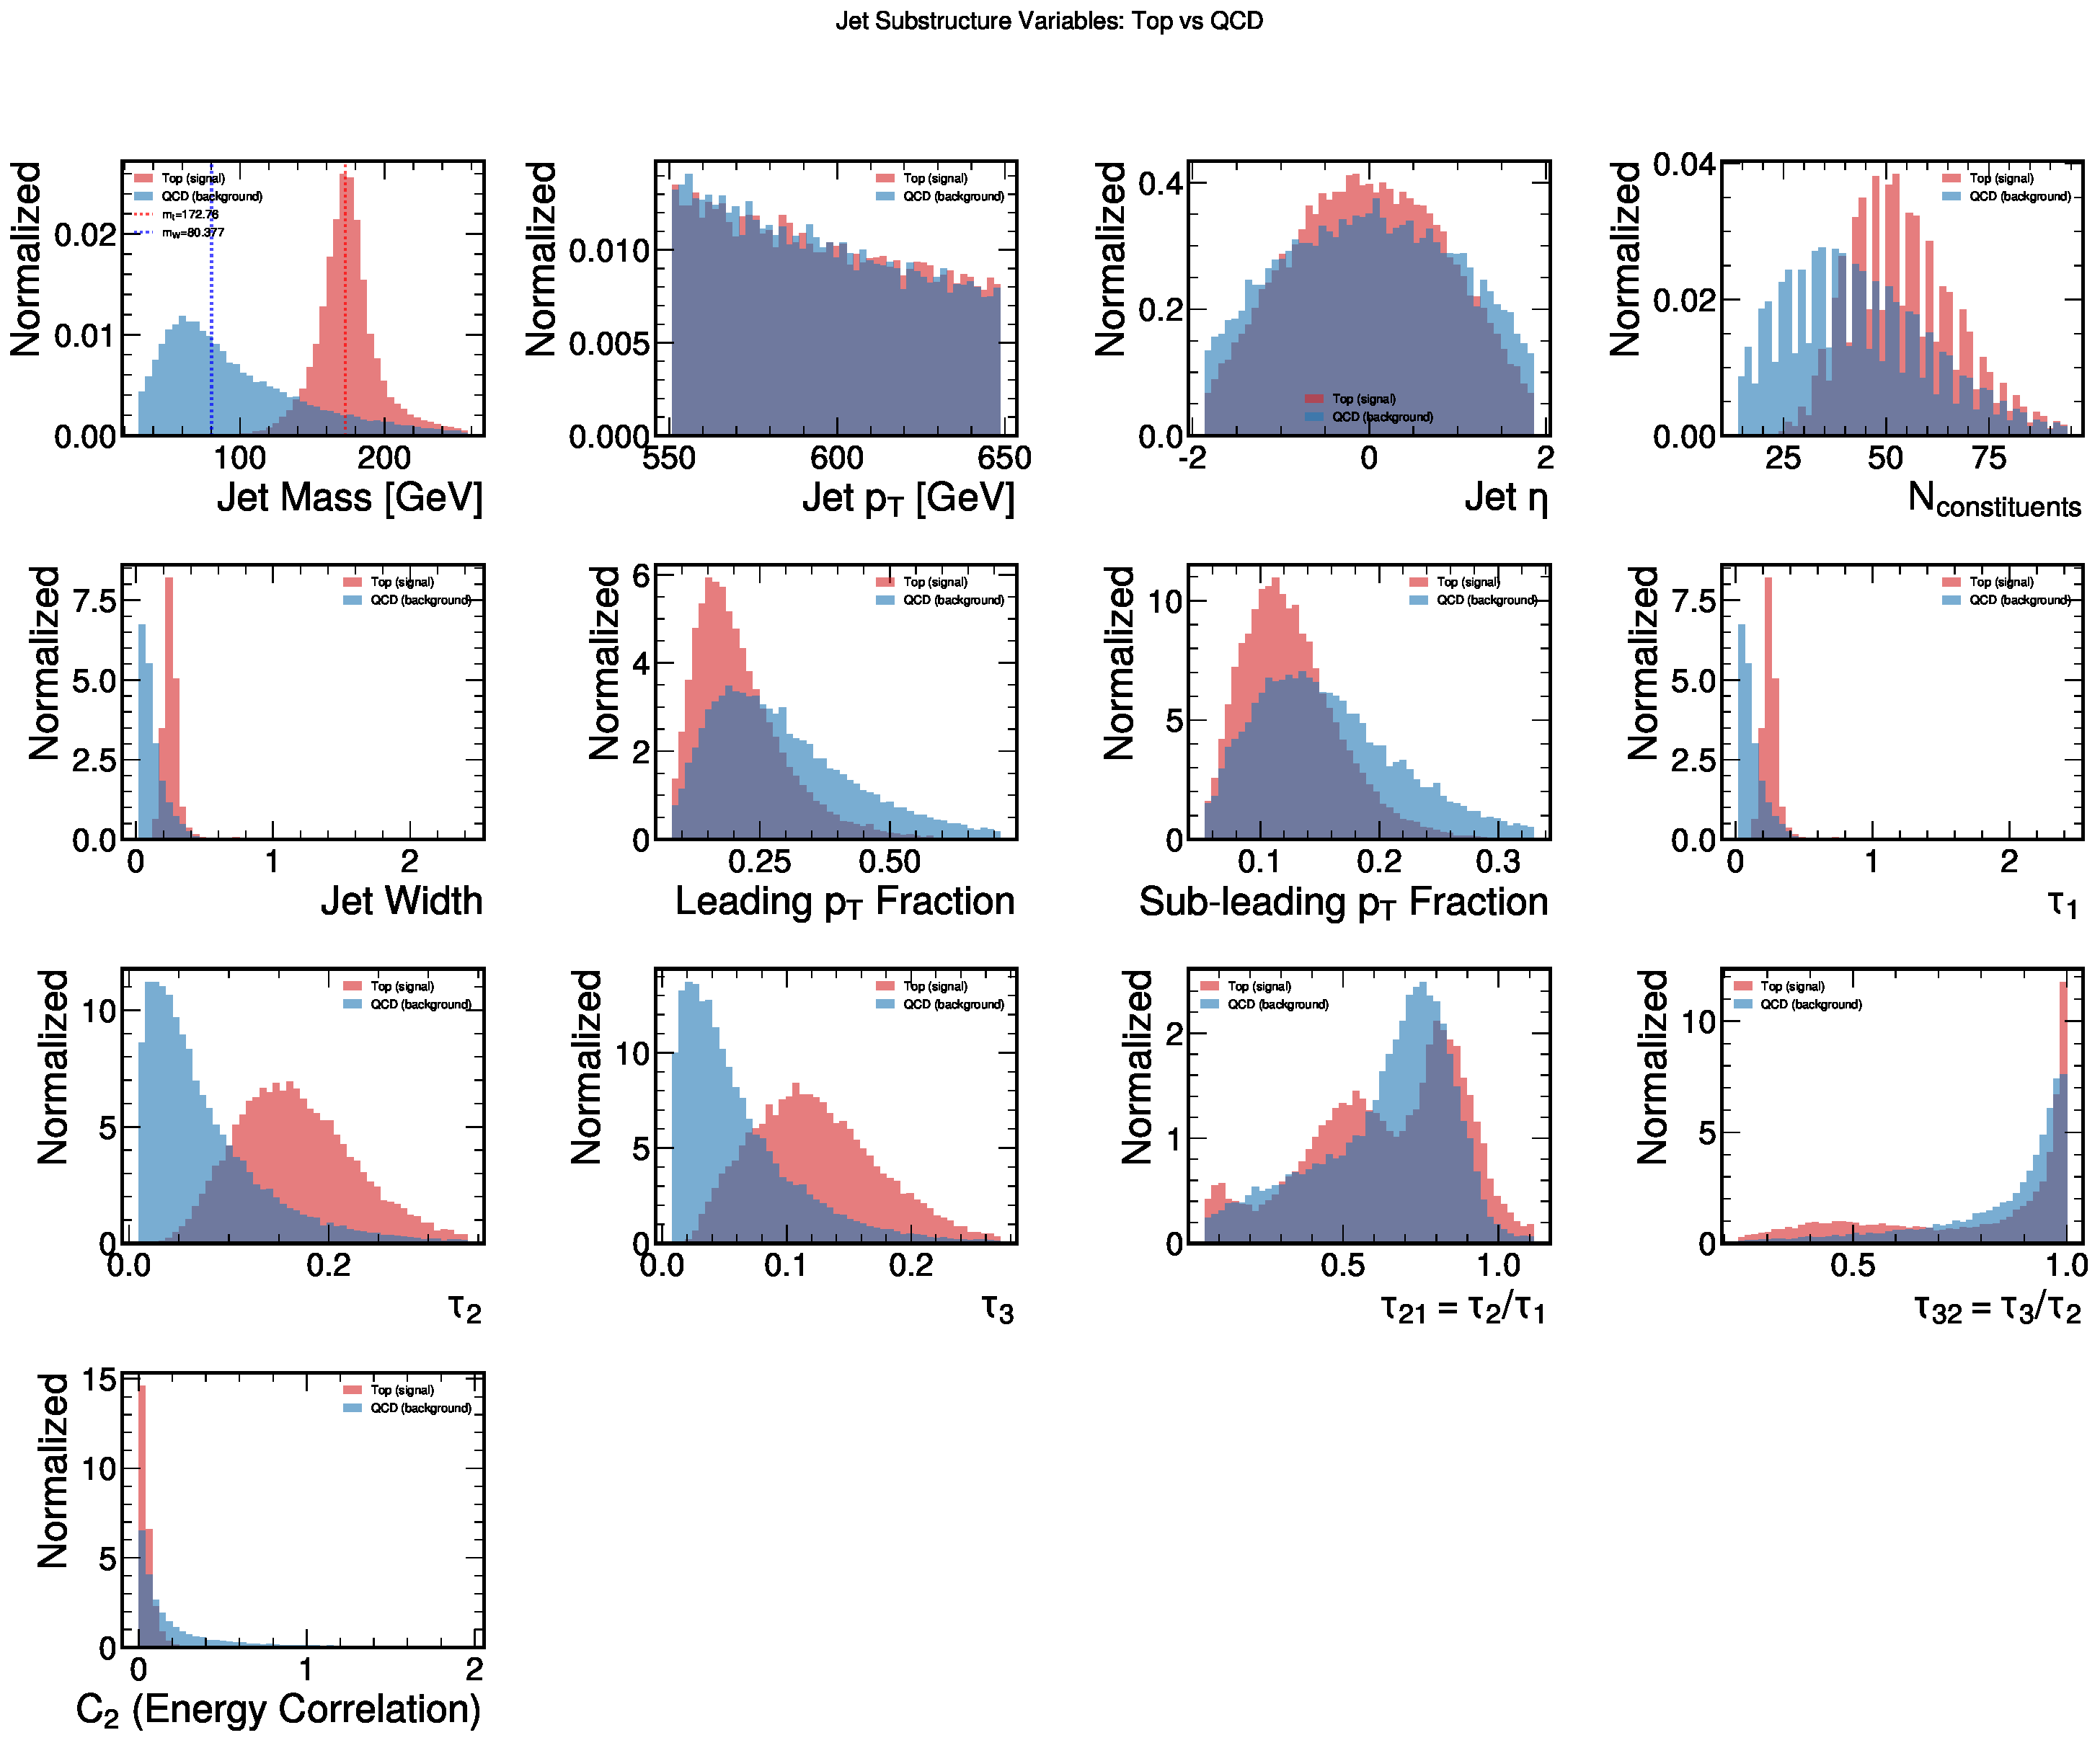
\includegraphics[width=\textwidth]{jet_substructure.pdf}
\caption{Distributions of the thirteen engineered jet-substructure
observables for top (signal) and QCD (background) jets on the test set. The
jet mass peaks at $m_t$ for top jets; $\tau_{32}$ and the constituent
multiplicity also separate the classes, as expected from physics.}
\label{fig:substructure}
\end{figure}

\begin{figure}[htbp]
\centering
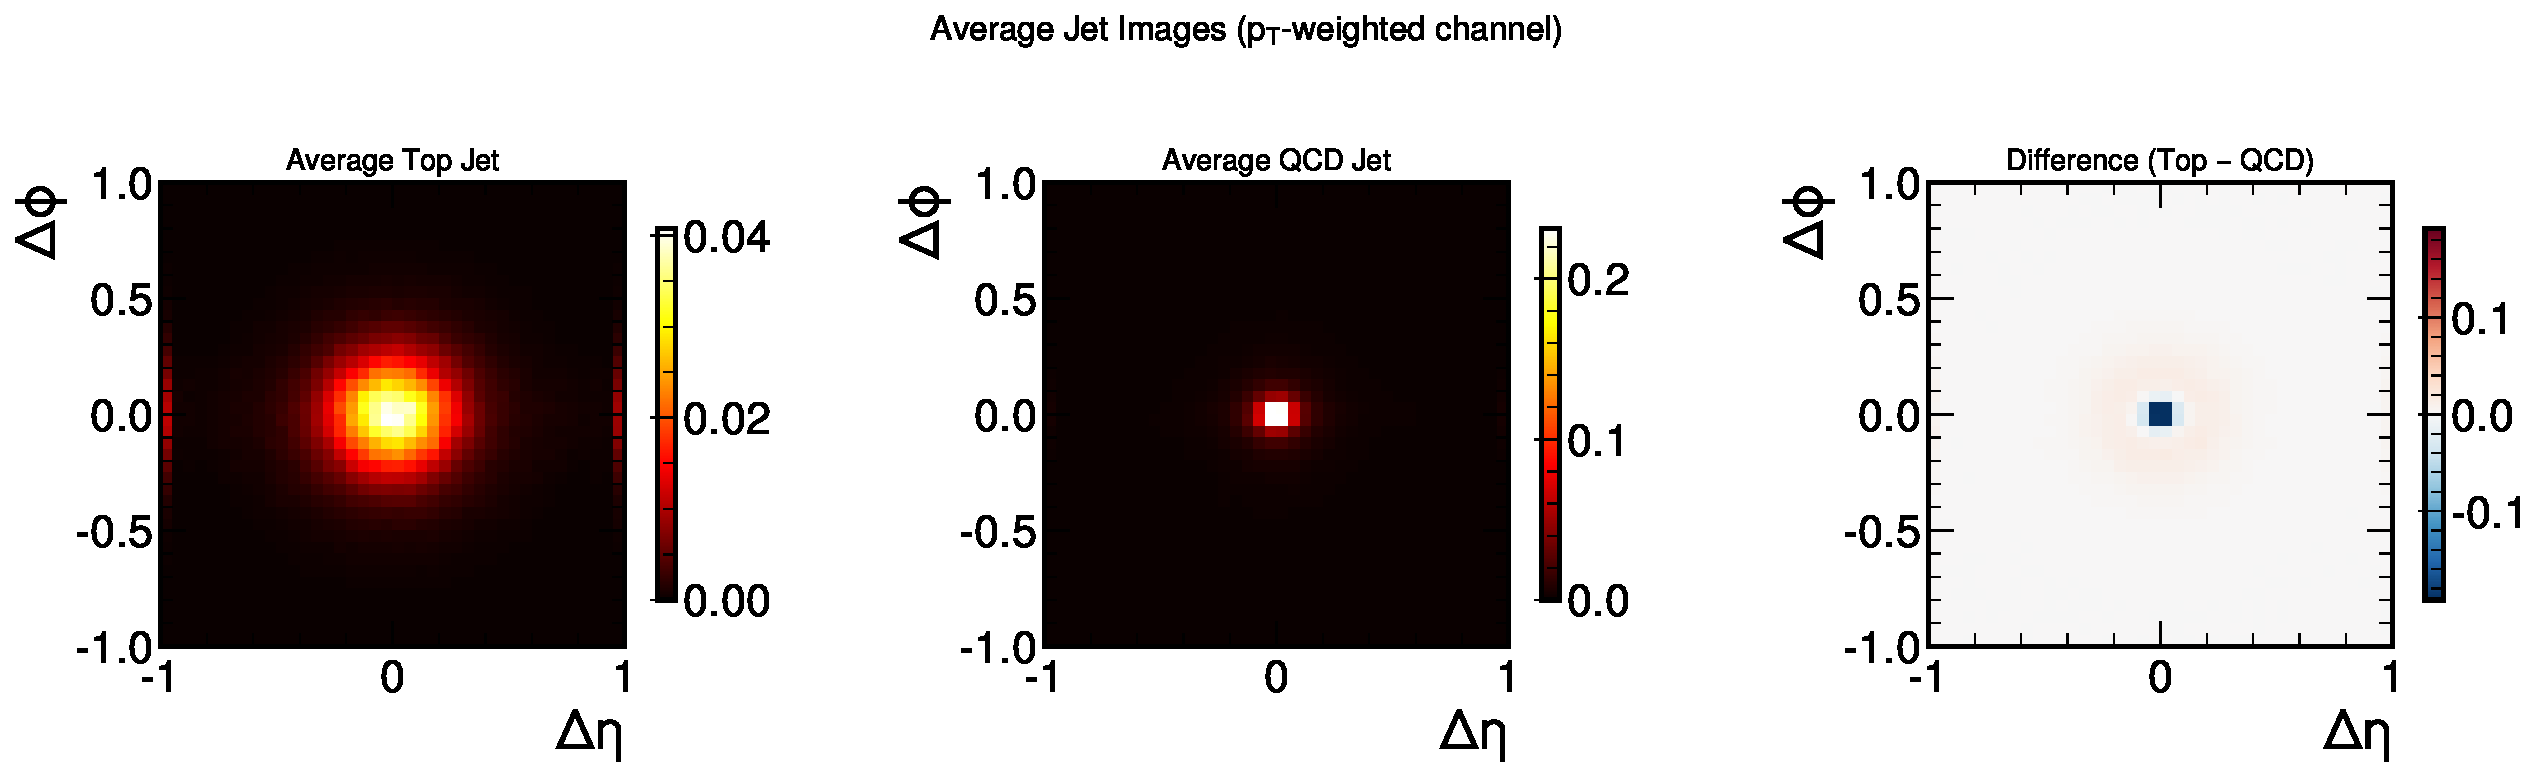
\includegraphics[width=\textwidth]{average_jet_images.pdf}
\caption{Average $p_T$-weighted jet images for top jets (left), QCD jets
(centre) and their difference (right). The three-prong structure of the
hadronic top decay is visible in the difference panel.}
\label{fig:avg_images}
\end{figure}

\subsection{Model comparison}
Table~\ref{tab:model_comparison} reports the headline performance of the four
models, and Figure~\ref{fig:roc} shows the ROC curves and background
rejection versus signal efficiency. The Particle Transformer achieves the
best discrimination (AUC $=0.978$, background rejection
$1/\varepsilon_B\approx136$ at $\varepsilon_S=0.5$), followed by ParticleNet,
the CNN and the BDT. This reproduces the ordering reported in the community
comparison~\citep{kasieczka2019landscape}; the absolute values sit slightly
below the published saturation values because we train on a subset rather
than the full $1.2\times10^{6}$ jets.

\IfFileExists{../../../results/comparison_table.tex}
  {\input{../../../results/comparison_table.tex}}
  {\emph{(comparison table generated by the pipeline)}}

\begin{figure}[htbp]
\centering
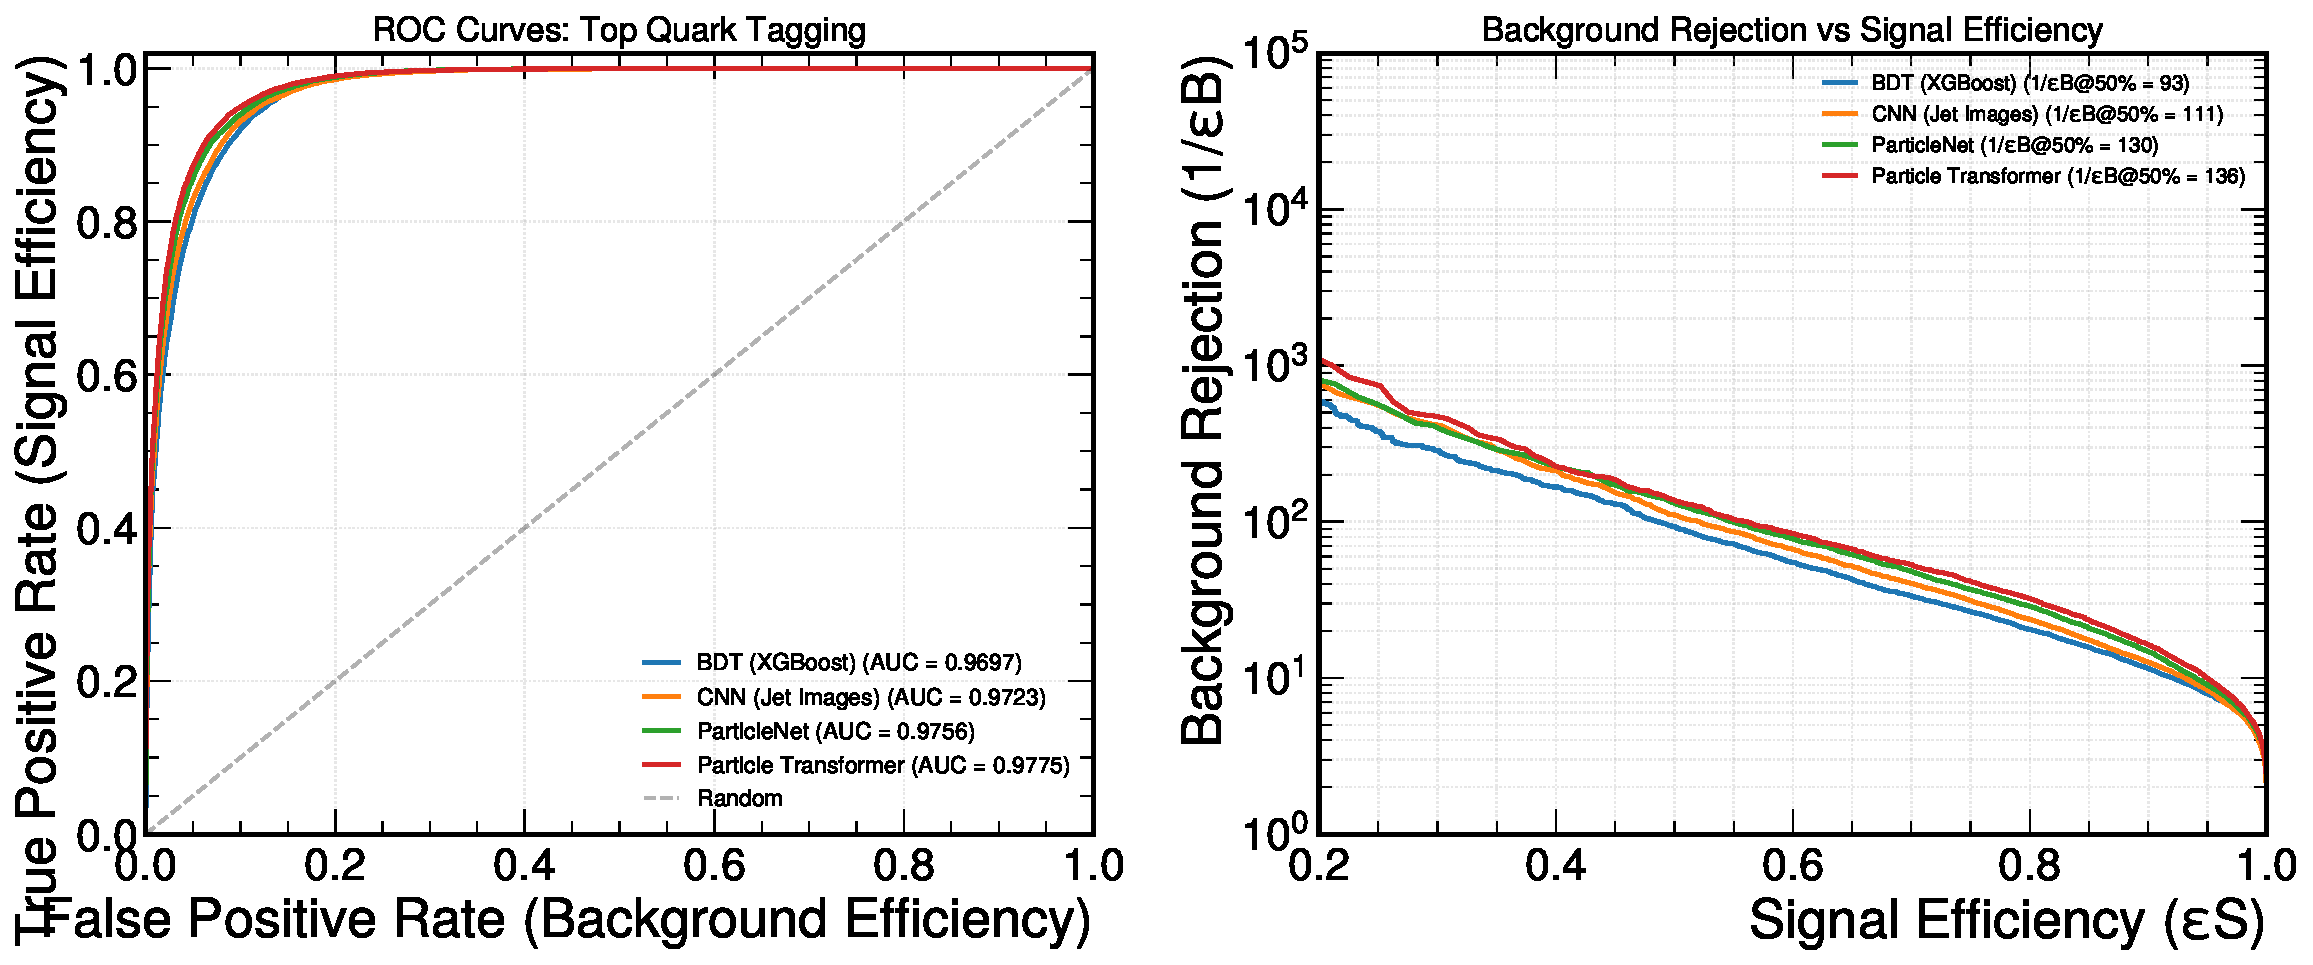
\includegraphics[width=\textwidth]{roc_comparison.pdf}
\caption{Left: ROC curves for the four models on the test set. Right:
background rejection $1/\varepsilon_B$ as a function of signal efficiency
$\varepsilon_S$. The Particle Transformer (red) is best across the range.}
\label{fig:roc}
\end{figure}

Figure~\ref{fig:scores} shows the classifier-score distributions and
Figure~\ref{fig:confusion} the confusion matrices at a threshold of $0.5$;
both confirm clean signal/background separation for all models, sharpest for
the deep architectures.

\begin{figure}[htbp]
\centering
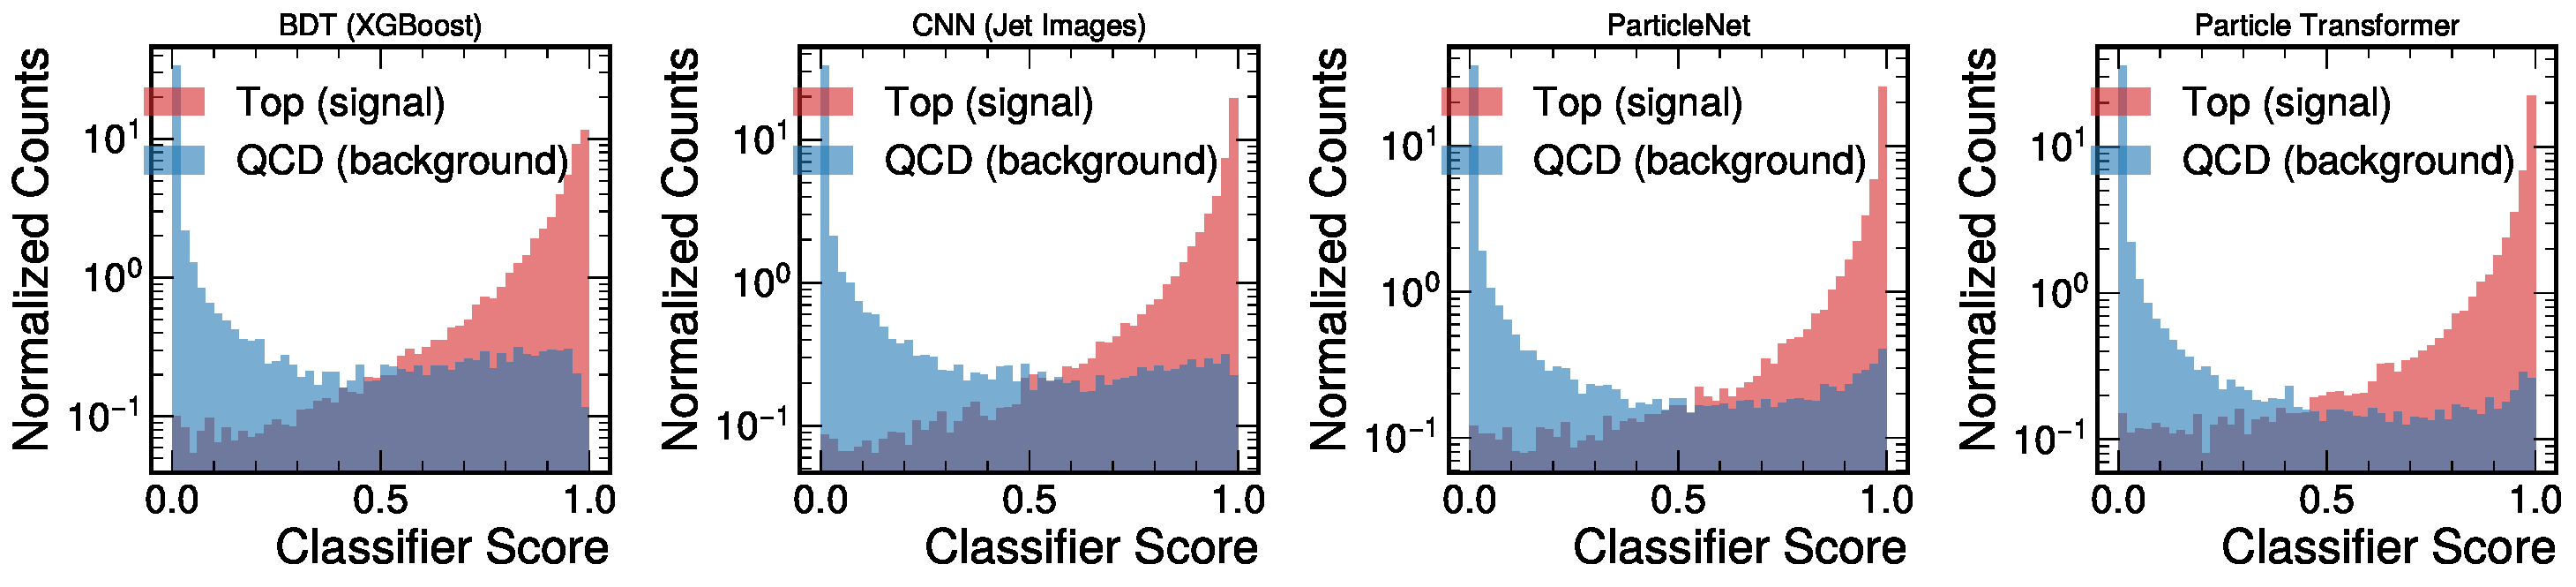
\includegraphics[width=\textwidth]{score_distributions.pdf}
\caption{Classifier-score distributions for top (red) and QCD (blue) jets.
Well-separated peaks near $0$ and $1$ indicate strong discrimination.}
\label{fig:scores}
\end{figure}

\begin{figure}[htbp]
\centering
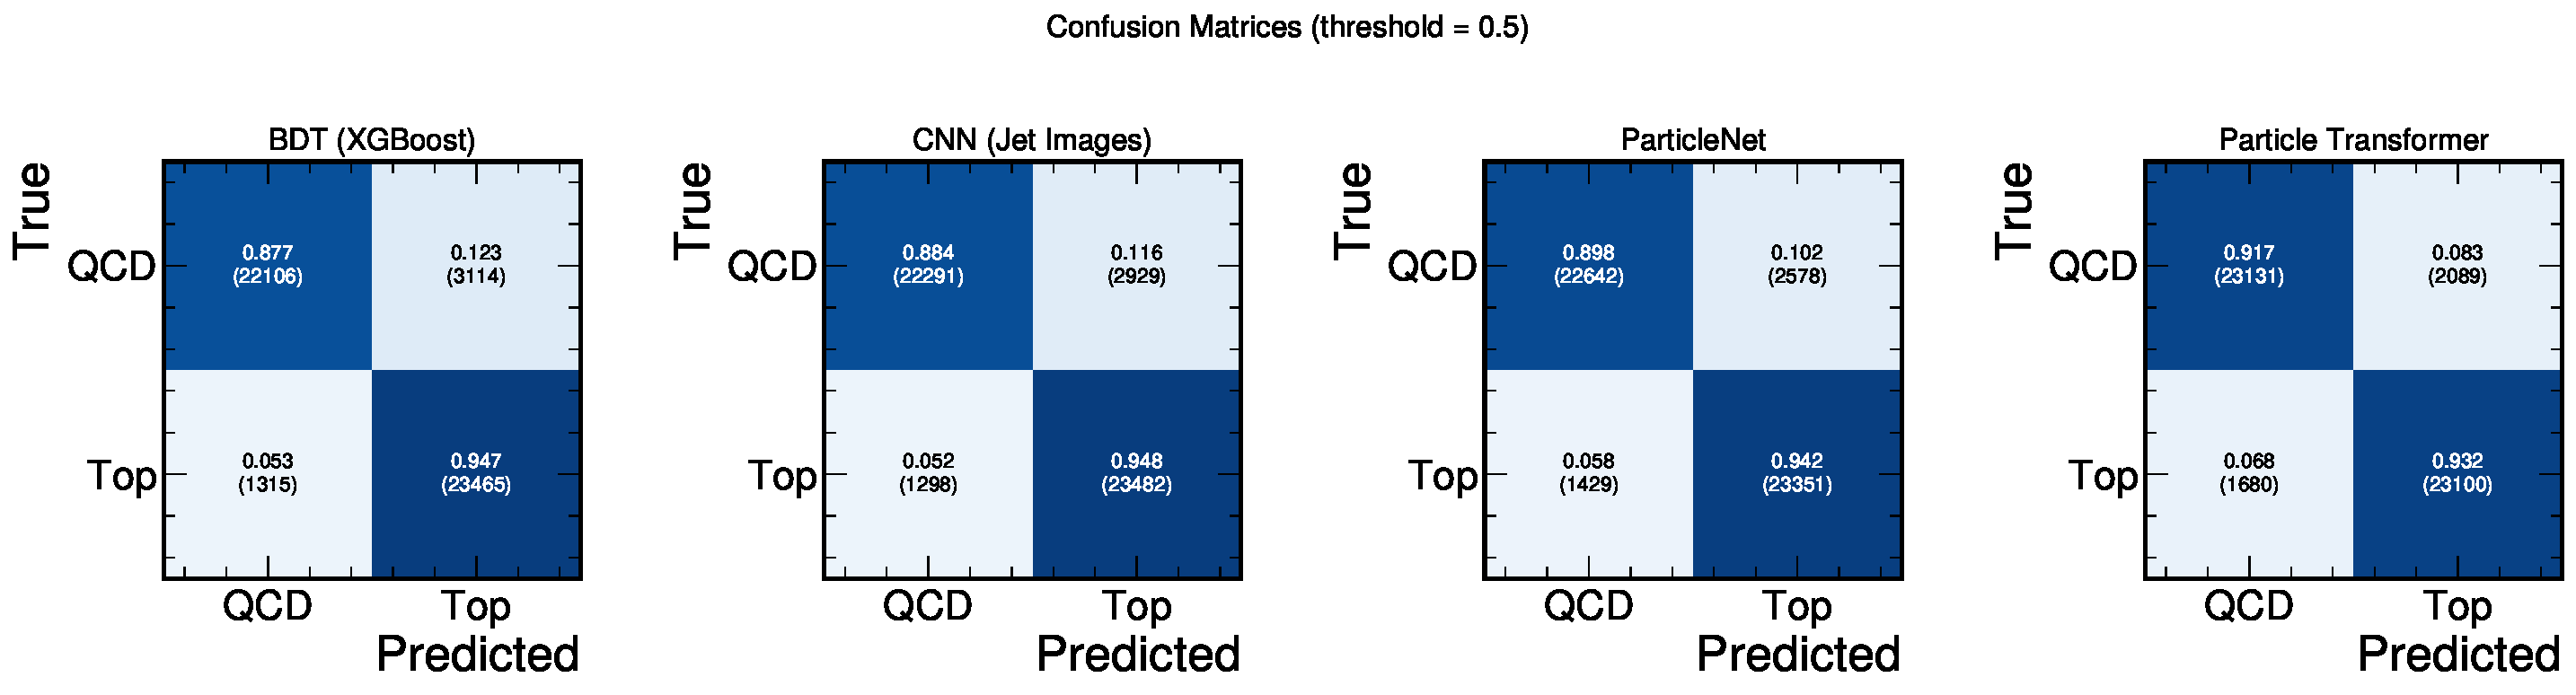
\includegraphics[width=\textwidth]{confusion_matrices.pdf}
\caption{Confusion matrices (normalised) at a decision threshold of $0.5$.}
\label{fig:confusion}
\end{figure}

\section{Data-Efficiency Study}
\label{sec:res_efficiency}

Figure~\ref{fig:learning} shows the test AUC and background rejection as a
function of the training-set size $N_{\text{train}}$. Three findings stand
out:
\begin{enumerate}
    \item \textbf{The BDT is the most data-efficient model.} Its AUC rises by
    under one percent (from $0.961$ to $0.968$) across the whole
    $5$k--$50$k range; engineered features short-circuit much of what the
    deep models must learn from data.
    \item \textbf{The deep models show a clear crossover.} The Particle
    Transformer is the \emph{weakest} model at $5$k jets (AUC $=0.949$) but
    the \emph{strongest} at $50$k ($0.974$), overtaking both the BDT and
    ParticleNet. Its slope is still positive at the largest size tested,
    consistent with the literature observation that it only saturates near
    $10^{6}$ jets~\citep{qu2022particletransformer}.
    \item \textbf{The CNN is intermediate}, gaining substantially with data
    ($0.947\rightarrow0.968$) but plateauing earlier than the
    permutation-equivariant graph and attention models.
\end{enumerate}
The practical message is that under a tight Monte~Carlo budget the simple,
interpretable BDT is competitive or better, whereas the attention model only
realises its advantage once enough data is available.

\begin{figure}[htbp]
\centering
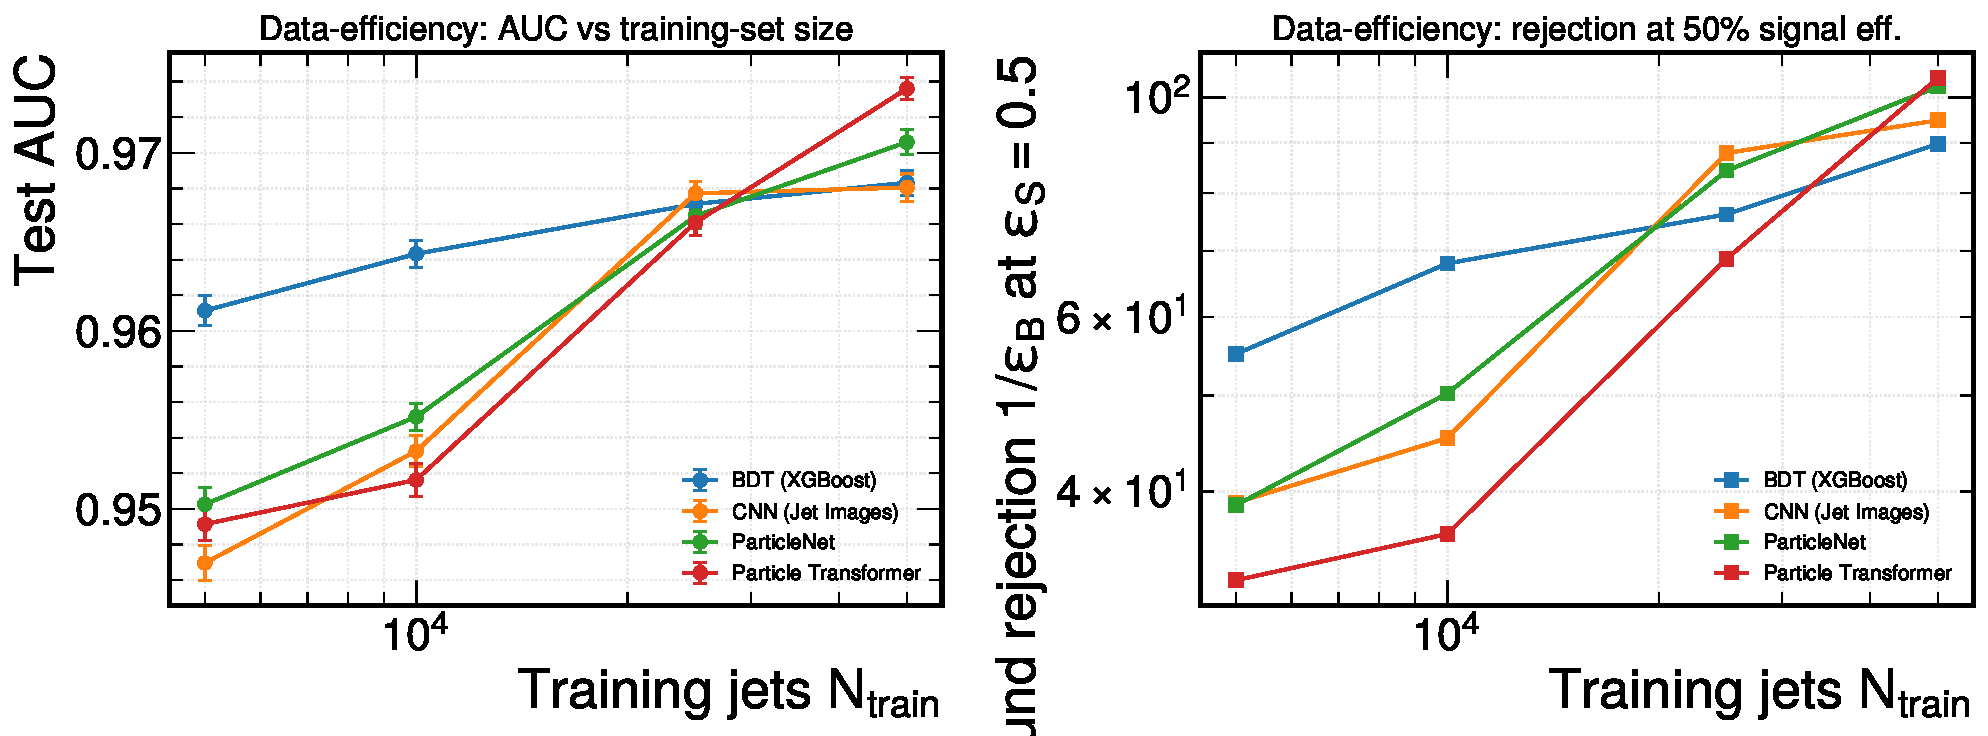
\includegraphics[width=\textwidth]{learning_curves.pdf}
\caption{Data-efficiency curves. Left: test AUC versus training-set size with
$1\sigma$ bootstrap error bars. Right: background rejection at
$\varepsilon_S=0.5$. The Particle Transformer rises from worst at $5$k jets
to best at $5\times10^{4}$, crossing the other models.}
\label{fig:learning}
\end{figure}

\section{Probability-Calibration Study}
\label{sec:res_calibration}

Figure~\ref{fig:calibration} shows the reliability diagrams and score
histograms, and Table~\ref{tab:calibration} reports the ECE, the fitted
temperature $T$ and the post-rescaling ECE. The key results are:
\begin{enumerate}
    \item \textbf{All models are mildly over-confident} (every fitted
    temperature satisfies $T>1$), in line with
    \citet{guo2017calibration}.
    \item \textbf{Ranking and calibration are decoupled.} The jet-image CNN
    is the worst-calibrated model by an order of magnitude (ECE $=0.078$,
    $T=1.54$) despite ranking only third on AUC, whereas the top-ranked
    Particle Transformer is comparatively well-calibrated (ECE $=0.012$). The
    BDT and ParticleNet are already well-calibrated (ECE $\approx0.007$).
    \item \textbf{Temperature scaling helps, but not uniformly.} A single
    scalar brings the BDT, ParticleNet and Particle Transformer to
    ECE\,$\lesssim0.008$, but only halves the CNN's error (to $0.064$): the
    CNN's miscalibration is structural and would need a richer recalibration
    such as isotonic regression.
\end{enumerate}

\begin{figure}[htbp]
\centering
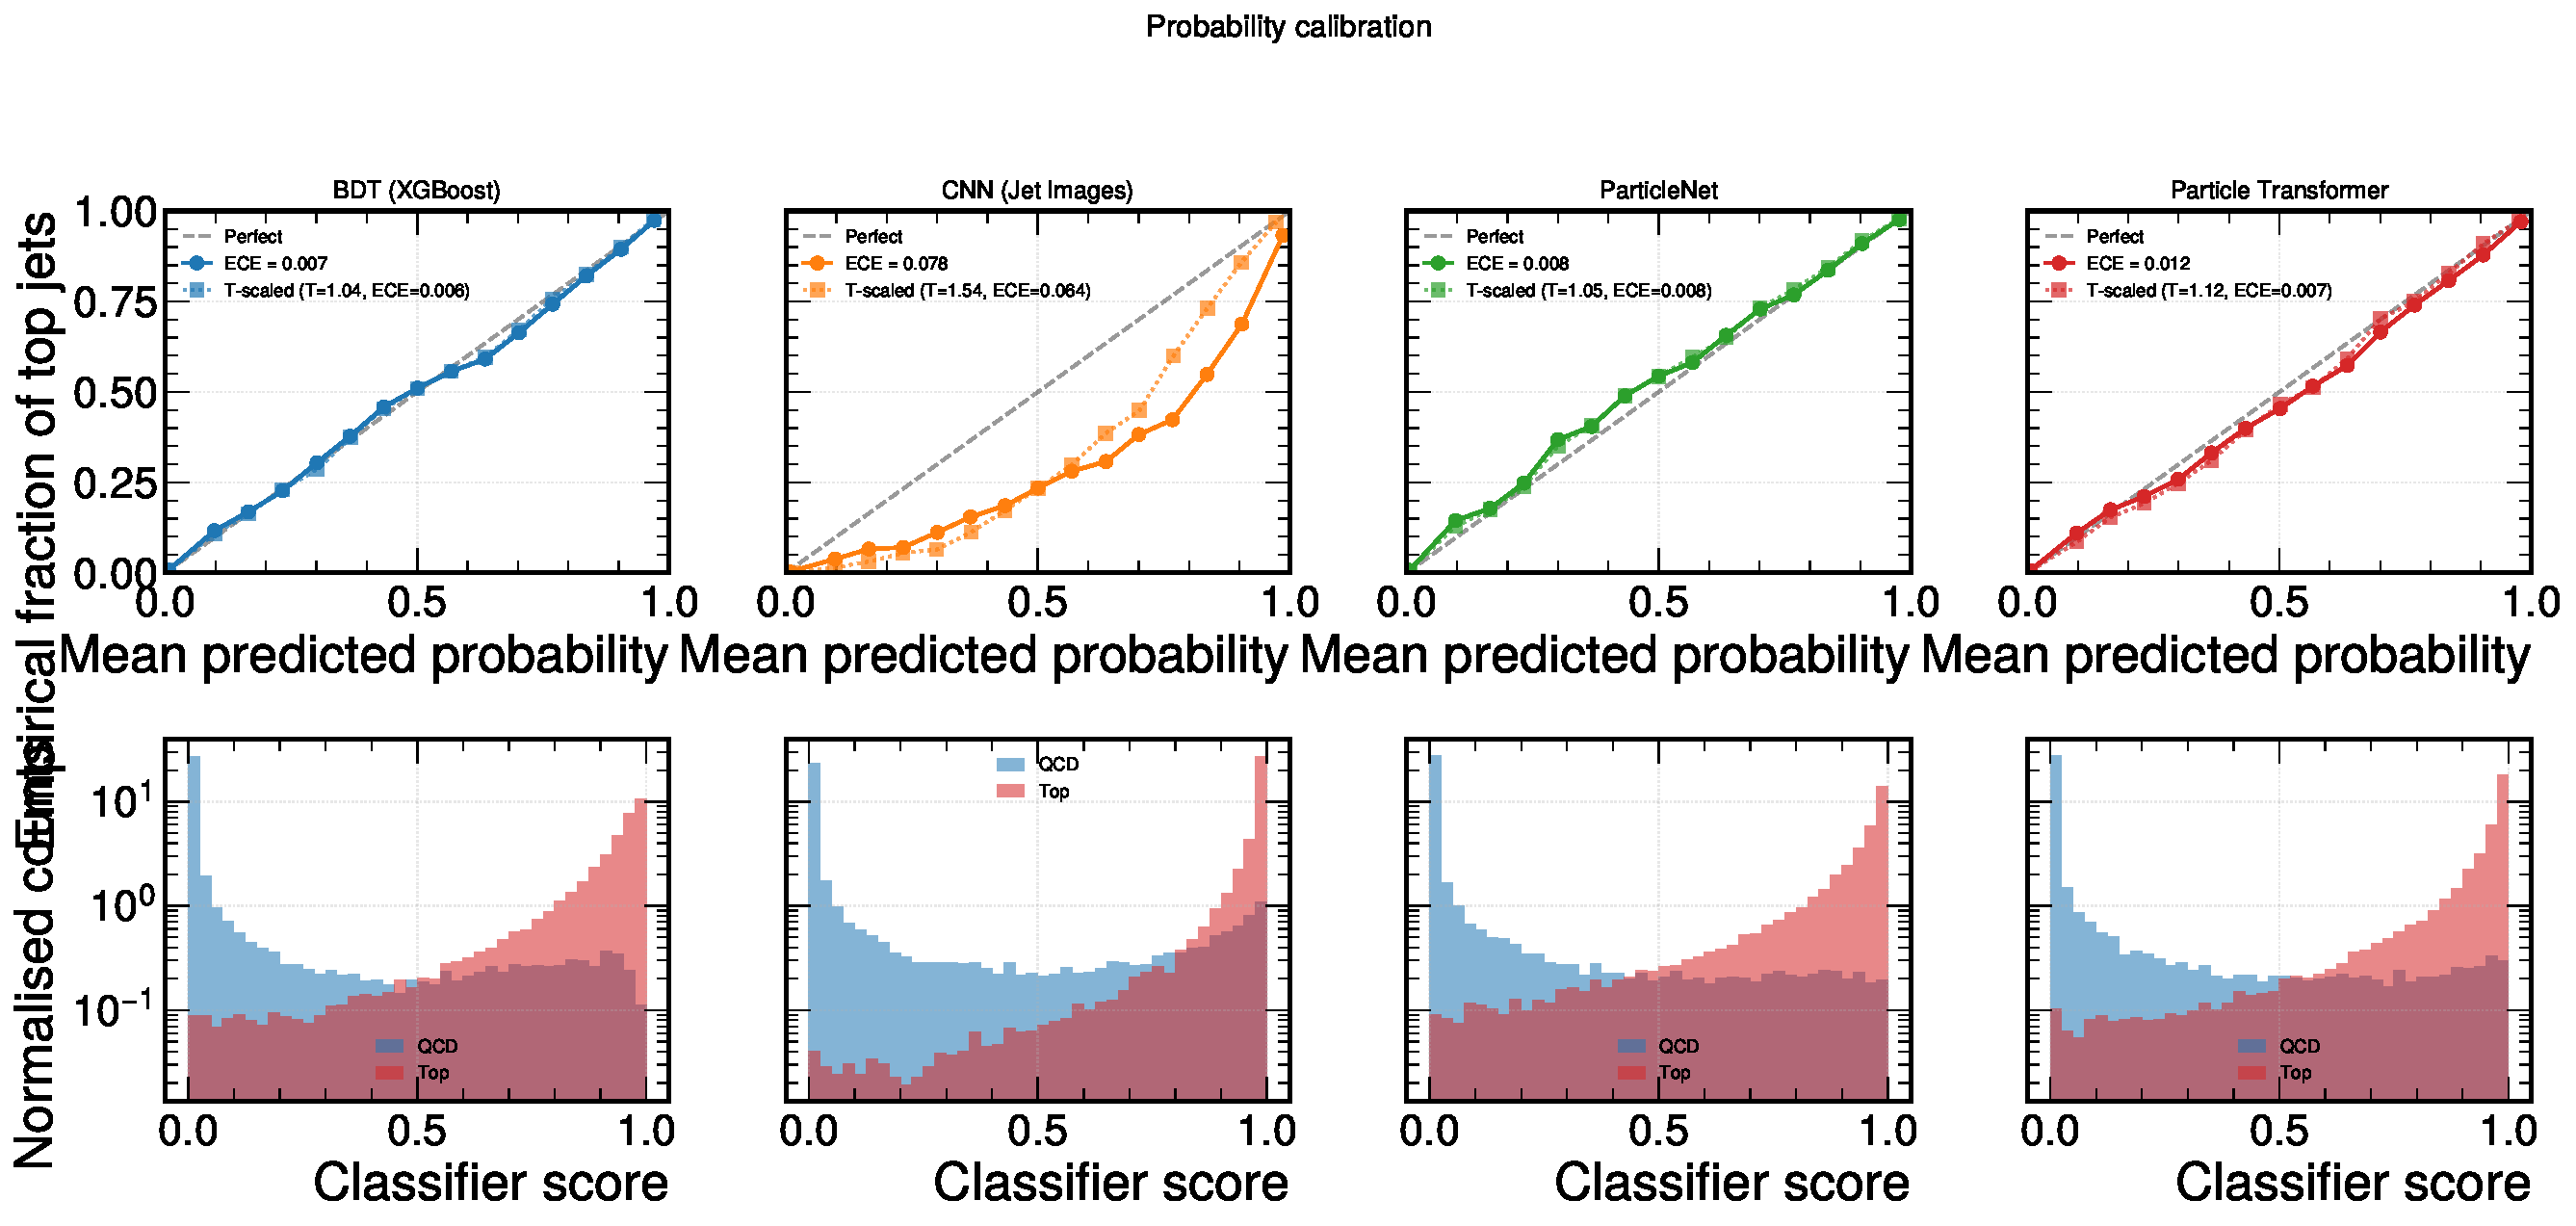
\includegraphics[width=\textwidth]{calibration.pdf}
\caption{Top: reliability diagrams for the four models (solid: raw scores;
dotted: after temperature scaling). Bottom: score histograms. The jet-image
CNN deviates most strongly from the diagonal.}
\label{fig:calibration}
\end{figure}

\begin{table}[htbp]
\centering
\caption{Test-set calibration at the $5\times10^{4}$-jet study endpoint. $T$
is the temperature fitted on the validation split; $\mathrm{ECE}_T$ is the
Expected Calibration Error after rescaling.}
\label{tab:calibration}
\ra{1.2}
\IfFileExists{../../../results/calibration_table.tex}
  {\input{../../../results/calibration_table.tex}}
  {\emph{(calibration table generated by the pipeline)}}
\end{table}

\section{Model Interpretability}
\label{sec:res_interpret}

Two views of \emph{why} the models work are useful. Figure~\ref{fig:bdt_imp}
shows the BDT feature importances: the jet mass (gain $118$), the
$1$-subjettiness $\tau_1$ ($89$) and the jet width ($76$) dominate, followed
by the constituent multiplicity ($15$) --- all sensitive to the larger mass,
girth and prong count of top jets. The canonical ratio $\tau_{32}$ ranks
lower (gain $7$): the boosted trees capture the prong information mainly
through the absolute $\tau_1$ and the jet width rather than the ratio, even
though $\tau_{32}$ is the cleaner discriminant at the distribution level
(Fig.~\ref{fig:substructure}).
Figure~\ref{fig:cls_attn} shows the class-token attention of the Particle
Transformer versus a constituent's angular distance $\Delta R$ from the jet
axis. For QCD jets the attention concentrates at small $\Delta R$ (a single
core), whereas for top jets it is spread to much larger $\Delta R$, reflecting
the broader, multi-pronged energy flow of the top decay. The model has
learned to attend to the peripheral radiation that carries the top signature.

\begin{figure}[htbp]
\centering
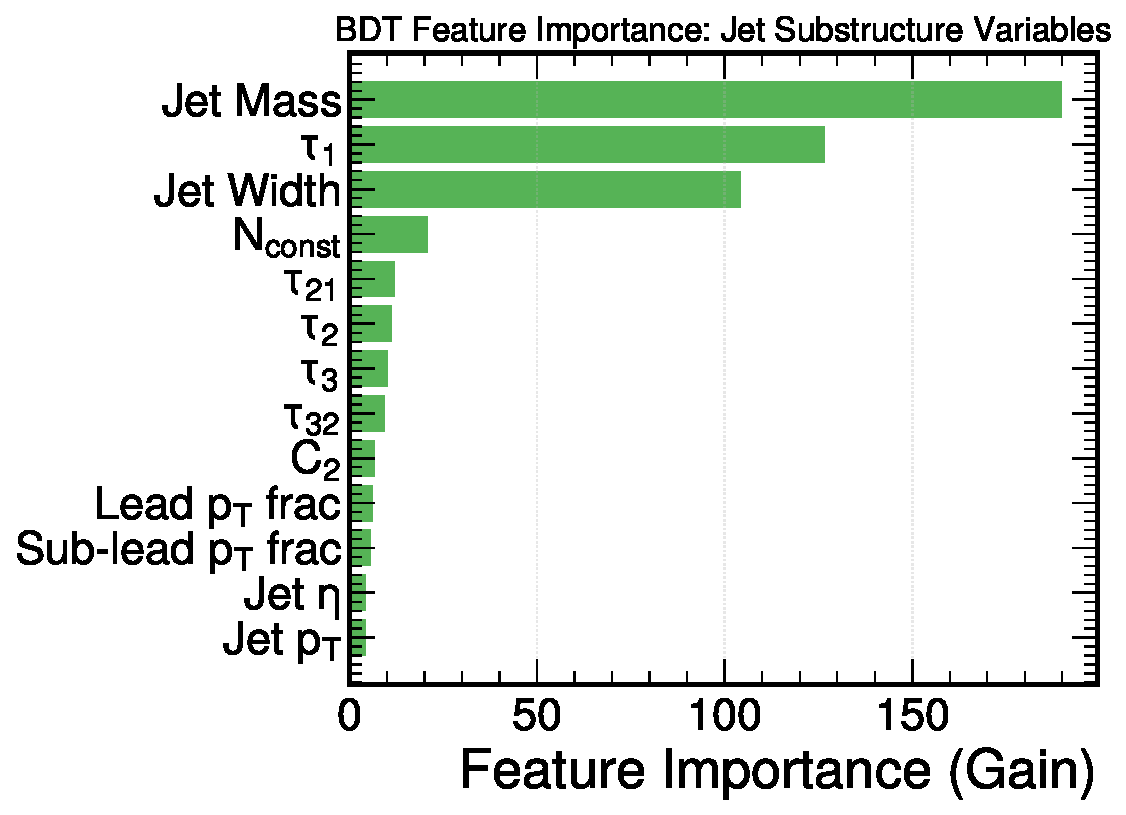
\includegraphics[width=0.8\textwidth]{bdt_importance.pdf}
\caption{Gain-based feature importance of the BDT. The jet mass, $\tau_1$
and jet width dominate, followed by the constituent multiplicity.}
\label{fig:bdt_imp}
\end{figure}

\begin{figure}[htbp]
\centering
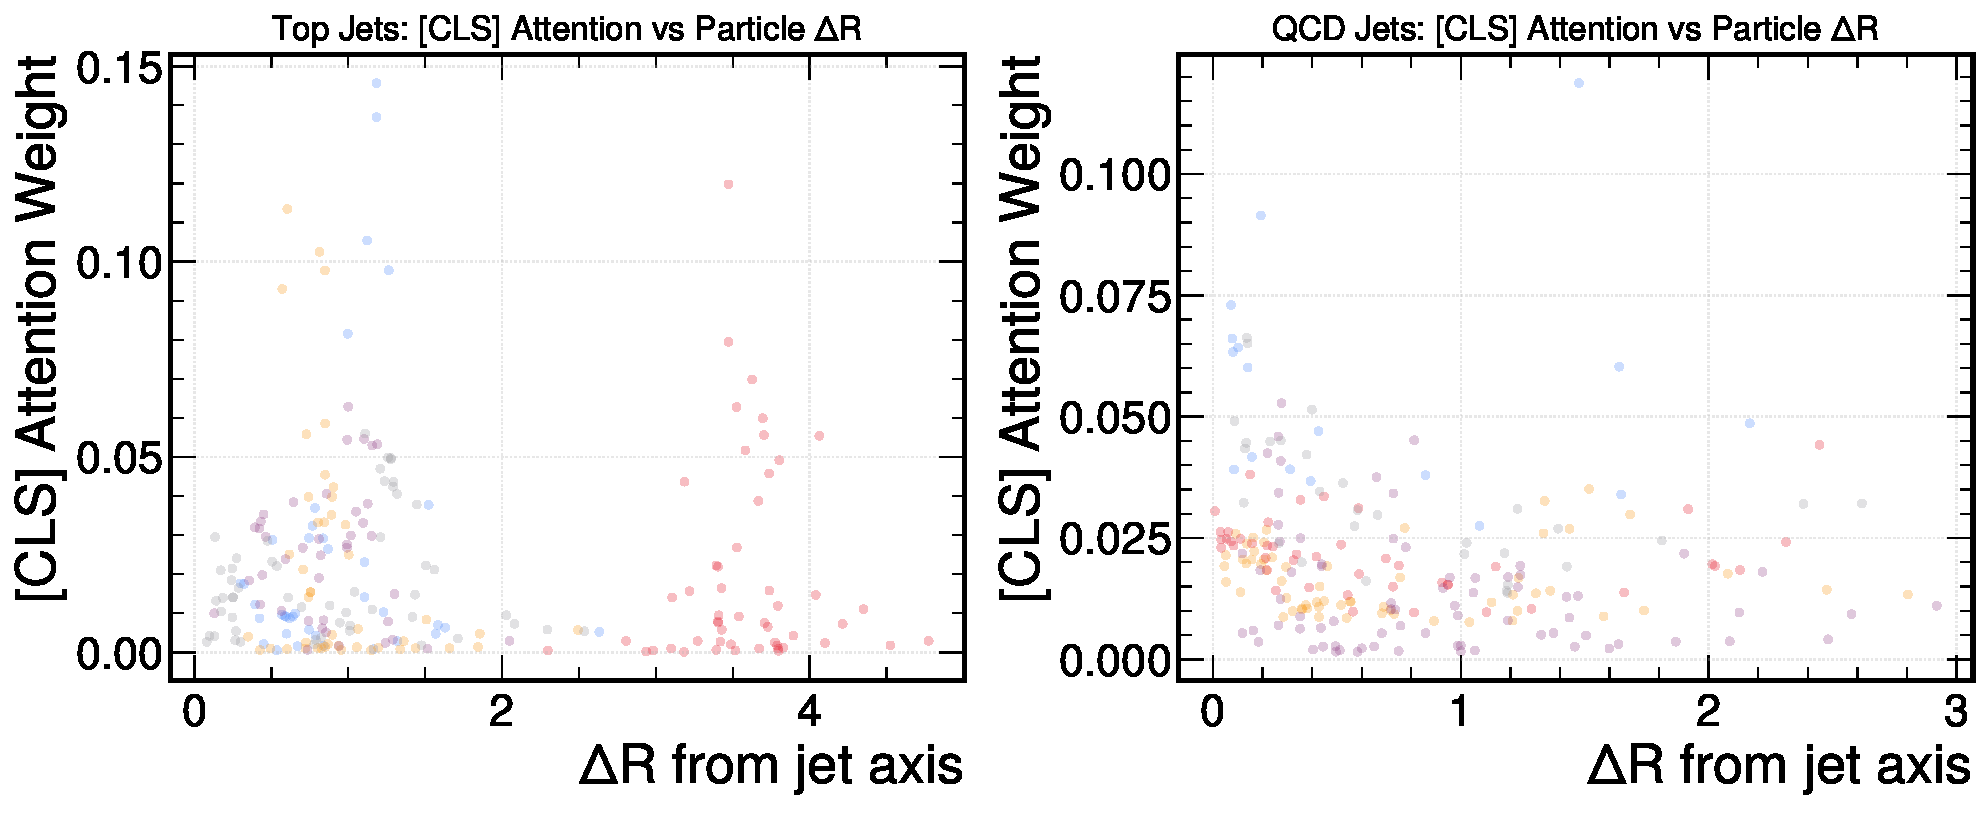
\includegraphics[width=\textwidth]{cls_attention.pdf}
\caption{Class-token attention weight of the Particle Transformer versus the
constituent angular distance $\Delta R$ from the jet axis, for top jets
(left) and QCD jets (right). Top jets draw attention to larger $\Delta R$,
matching their multi-prong structure.}
\label{fig:cls_attn}
\end{figure}

\section{Summary of Findings}
\label{sec:res_summary}

\begin{enumerate}
    \item The pipeline reproduces the established ordering Particle
    Transformer $>$ ParticleNet $>$ CNN $>$ BDT, with the Particle
    Transformer reaching AUC $=0.978$.
    \item Data efficiency separates the models sharply: the BDT is best in
    the small-data regime, while the deep models overtake it as data grows,
    producing a clear crossover.
    \item Ranking power and calibration are decoupled: the CNN is the
    worst-calibrated model despite a mid-pack ranking, and temperature
    scaling fixes every model except the CNN.
\end{enumerate}
                     % Chapter 4: Results and Discussion
	\chapter{Conclusions and Future Work}
\label{chap:conclusions}

\section{Conclusions}
\label{sec:conclusions}

This thesis built a transparent, reproducible top-tagging pipeline and used
it to compare four classifiers --- a boosted decision tree on engineered
features, a jet-image CNN, the ParticleNet graph network and the Particle
Transformer --- on the public 14\,TeV Top-Quark Tagging Reference Dataset,
with a focus on data efficiency and probability calibration rather than on a
new record. Returning to the objectives of
Chapter~\ref{chap:introduction}, the study reached the following
conclusions.

\begin{enumerate}
    \item \textbf{The established ordering is reproduced.} Under identical
    preprocessing and a modest budget, the Particle Transformer is best
    (AUC $=0.978$, $1/\varepsilon_B\approx136$ at $\varepsilon_S=0.5$),
    followed by ParticleNet, the CNN and the BDT, matching the community
    benchmark.
    \item \textbf{Data efficiency separates the models.} The BDT is the most
    data-efficient and is the strongest model at the smallest training size,
    but it is overtaken by the deep models as data grows. The Particle
    Transformer in particular rises from the weakest model at $5\times10^{3}$
    jets to the strongest at $5\times10^{4}$, a clear crossover with direct
    practical implications for low-statistics analyses.
    \item \textbf{Ranking and calibration are decoupled.} The highest-AUC
    model (the Particle Transformer) is comparatively well-calibrated,
    whereas the jet-image CNN --- only third on AUC --- is the
    worst-calibrated by an order of magnitude. A single-parameter temperature
    rescaling restores good calibration for the BDT, ParticleNet and the
    transformer, but only partially corrects the CNN. A high AUC therefore
    does not by itself license the use of a model's score as a probability.
    \item \textbf{World-class benchmarks are reproducible on free hardware.}
    The entire study was run on a free cloud GPU using open data and open
    tools, with automatic checkpointing and resumption, demonstrating that
    such work is accessible to students in resource-constrained settings.
\end{enumerate}

\section{Limitations}
\label{sec:limitations}

The study used subsamples of up to $5\times10^{4}$ jets rather than the full
$1.2\times10^{6}$, so absolute performances are slightly below the published
saturation values; the trends, not the records, are the contribution. The
reference dataset contains no pile-up and uses a single detector
parametrisation, so detector robustness and high-luminosity behaviour are not
addressed. Each architecture was trained with a fixed, modest configuration
rather than an exhaustive hyper-parameter search, and four models, while
representative, are not exhaustive.

\section{Future Work}
\label{sec:future}

Several extensions follow naturally from this work:
\begin{enumerate}
    \item \textbf{Scale up.} Repeat the data-efficiency sweep up to the full
    $1.2\times10^{6}$ jets on a larger GPU to locate precisely where the
    transformer overtakes ParticleNet by a statistically significant margin.
    \item \textbf{Richer recalibration.} Compare temperature scaling with
    non-parametric isotonic regression, particularly for the CNN whose
    miscalibration temperature scaling does not fully remove.
    \item \textbf{Robustness.} Study calibration and discrimination under
    simulated pile-up and detector smearing, which is where calibration
    matters most for real analyses.
    \item \textbf{More architectures.} Add a Deep~Sets baseline and a
    Lorentz-equivariant network~\citep{gong2022lorentznet} to the comparison.
    \item \textbf{Uncertainty quantification.} Use deep ensembles or
    Monte-Carlo dropout to attach predictive uncertainties to the tagger
    scores.
\end{enumerate}

In summary, this project shows that asking \emph{how much data} and
\emph{how trustworthy the probabilities are}, rather than only \emph{how
high the AUC}, yields a more complete and more useful picture of deep
jet-tagging models --- and that this picture can be obtained reproducibly on
freely available hardware.
                 % Chapter 5: Conclusions


	%% ============================================================
	%% APPENDICES
	%% ============================================================
	\appendix
	\chapter{Reproducibility and Supplementary Material}
\label{chap:appendix_a}

\section{Code and Data Availability}
\label{sec:availability}

The complete pipeline --- data loading, feature engineering, the four models,
training, evaluation and all plotting --- is released as open source at
\begin{center}
\url{https://github.com/ramc77/fyp-jet-tagging}
\end{center}
The dataset is the public Top-Quark Tagging Reference
Dataset~\citep{kasieczka2019dataset}, available from Zenodo
(\url{https://zenodo.org/records/2603256}).

\section{How to Reproduce the Results}
\label{sec:reproduce}

On a machine with Python~3.11 the headline results and study are reproduced
with:
\begin{verbatim}
python3 -m venv particle_venv
source particle_venv/bin/activate
pip install -r requirements.txt
python3 download_data.py --yes        # fetch the dataset
python3 run_full_pipeline.py          # train + evaluate all four models
python3 run_study.py                  # data-efficiency + calibration sweep
\end{verbatim}
A Google Colaboratory notebook (\texttt{notebooks/FYP\_Colab.ipynb}) runs the
same pipeline on a free T4 GPU and downloads the results. Every training stage
checkpoints after each epoch and resumes automatically, so a run may be
interrupted and continued.

\section{Training Configuration}
\label{sec:config}

\begin{table}[htbp]
\centering
\caption{Principal hyper-parameters of the four models.}
\label{tab:hyperparams}
\ra{1.2}
\begin{tabular}{@{}lll@{}}
\toprule
\textbf{Model} & \textbf{Key settings} & \textbf{Parameters} \\
\midrule
BDT (XGBoost)        & 500 rounds, depth 7, lr 0.1   & $\sim$160 trees \\
CNN (jet images)     & 3 ResNet blocks, 64--256 ch.  & $1.26$\,M \\
ParticleNet          & 3 EdgeConv blocks, $k=16$     & $0.37$\,M \\
Particle Transformer & 3 blocks, 4 heads, dim 128    & $0.43$\,M \\
\bottomrule
\end{tabular}
\end{table}

All models minimise binary cross-entropy with the Adam/AdamW optimiser,
gradient clipping, a plateau learning-rate scheduler and early stopping on
the validation AUC, as detailed in Section~\ref{sec:training}.

\section{Training History}
\label{sec:history}

Figure~\ref{fig:history} shows the training and validation loss and AUC
curves for the three neural models, confirming smooth convergence without
significant over-fitting within the epoch budget.

\begin{figure}[htbp]
\centering
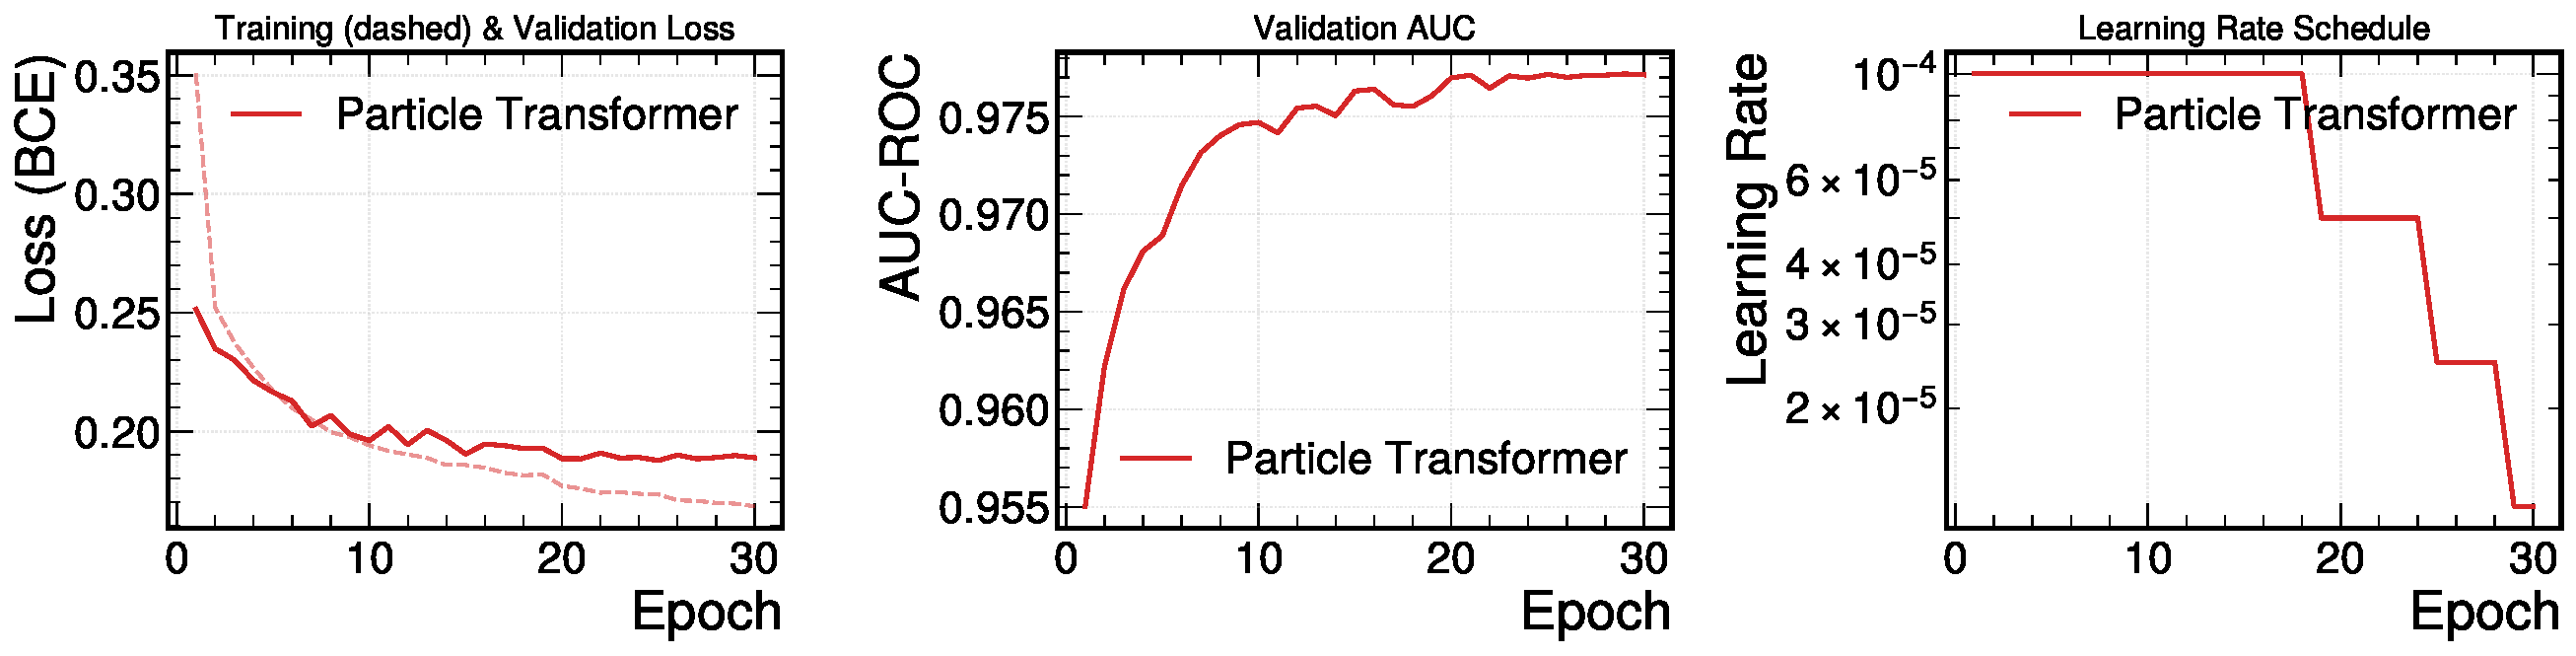
\includegraphics[width=\textwidth]{training_history.pdf}
\caption{Training/validation loss and validation AUC versus epoch for the
CNN, ParticleNet and Particle Transformer.}
\label{fig:history}
\end{figure}

\section{Transformer Attention Maps}
\label{sec:attnmaps}

Figure~\ref{fig:attnmaps} shows representative head-averaged self-attention
maps for top jets across the transformer layers, complementing the
class-token analysis in Section~\ref{sec:res_interpret}.

\begin{figure}[htbp]
\centering
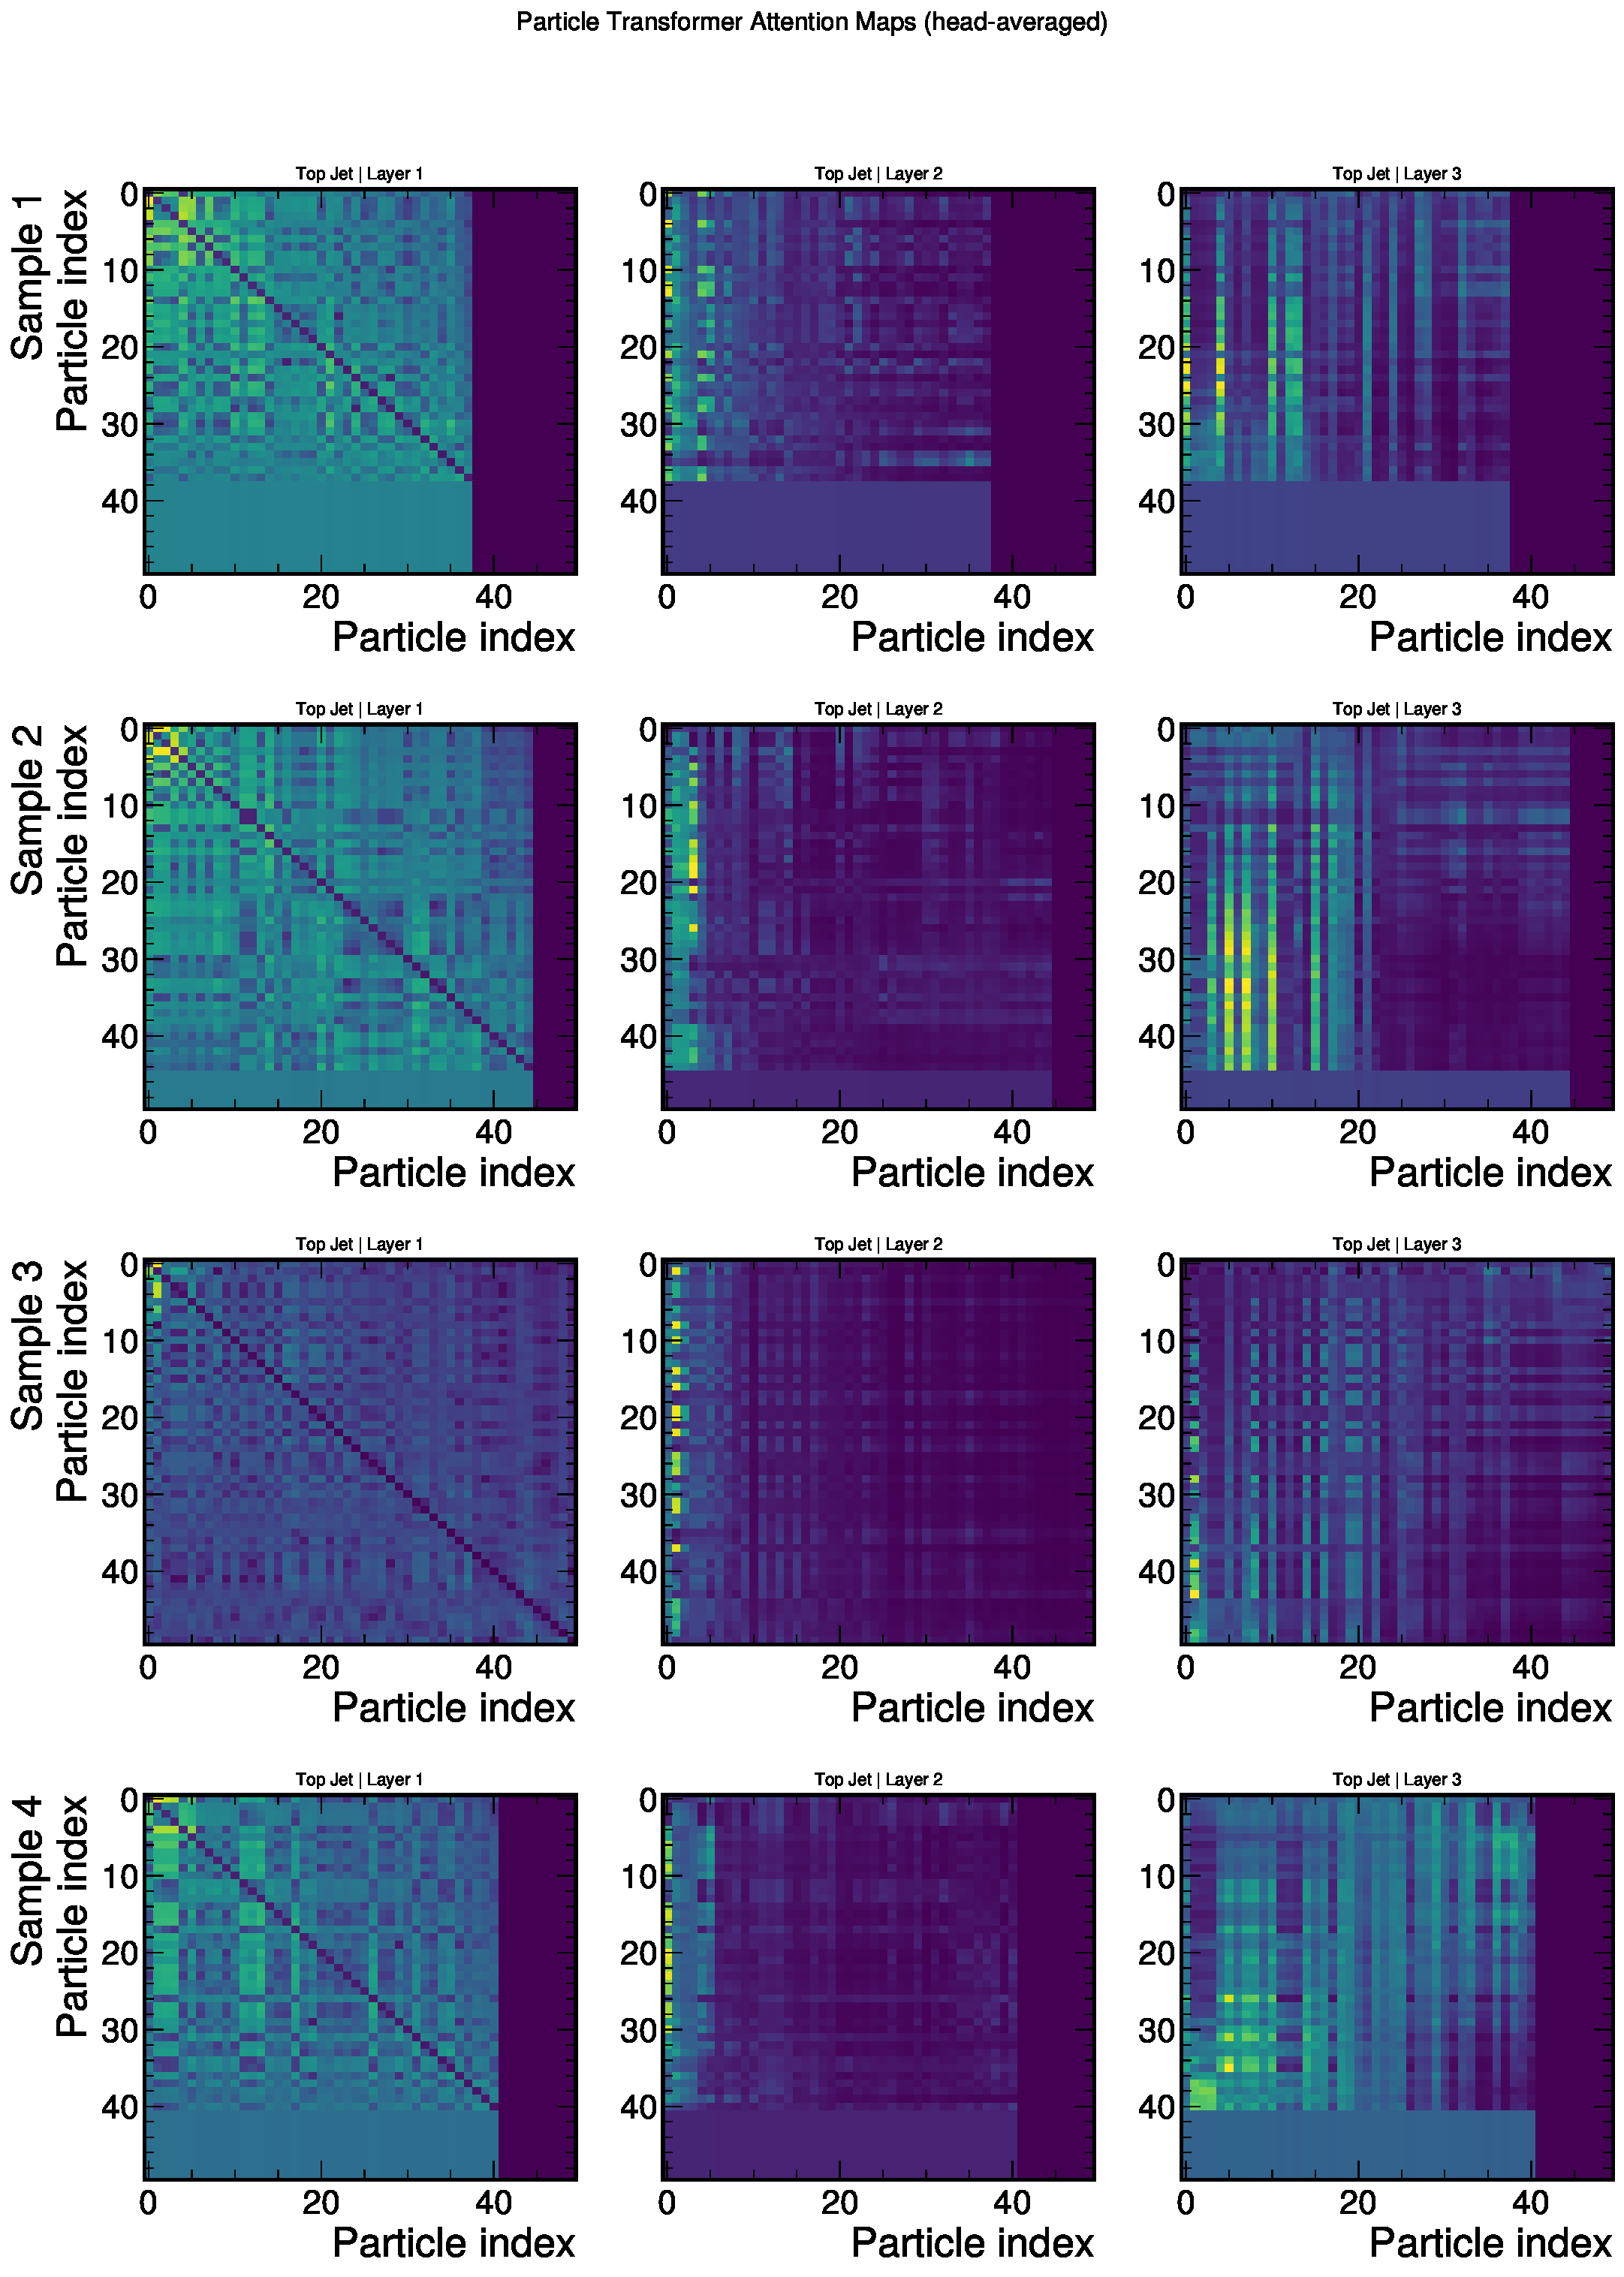
\includegraphics[width=0.9\textwidth]{attention_maps.pdf}
\caption{Head-averaged self-attention maps of the Particle Transformer for
sample top jets across the encoder layers. The padded (non-particle)
positions appear as uniform blocks.}
\label{fig:attnmaps}
\end{figure}
                   % Appendix A


	%% ============================================================
	%% BACK MATTER -- References and index.
	%% ============================================================
	{\backmatter
		\if@openright\cleardoublepage\else\clearpage\fi
		\bibliographystyle{bnb-plainnat}           % BNBWU bibliography style
		{\footnotesize\bibliography{references}}   % your .bib file(s)
		\printindex
	}

\end{document}

%%% The End %%%
